\documentclass[final,onecolumn]{IEEEtran}

% Required packages for math and citations
\usepackage{amsmath, amssymb, amsfonts}
\usepackage{physics}
\usepackage{cite}
\usepackage{datetime}
\usepackage{setspace}
\usepackage{totcount}
\usepackage{comment}
\usepackage{listings}
\usepackage{tikz}
\usetikzlibrary{calc,patterns,angles,quotes,decorations.pathmorphing}
% Load tikz before standard LaTeX packages like graphicx
\usepackage{graphicx}
\graphicspath{{../figures/}}
\usepackage[hidelinks]{hyperref}
\usepackage{float}
\usepackage{pdfpages}


\bibliographystyle{ieeetr}
\doublespacing

% --- Document Begins ---
\begin{document}

% --- Title Page ---
\begin{titlepage}
    \centering
    \vspace*{1in} % Moves the title block down by an inch

    {\huge{Analytical Modeling of Wind Turbine Dynamics\\[0.5em] Using Symbolic Lagrangian Mechanics}}\par

    \vspace{2em}

    {\Large Dinor Nallbani}\par

    \vfill

    \begin{tabular}{ l l }
        \textbf{Chair:} & Emmanuel Branlard \\
        \textbf{Date:}  & \today
    \end{tabular}

    \vfill
\end{titlepage}

% --- Abstract Page ---
\newpage
\begin{center}
    \textbf{ABSTRACT}
\end{center}
\vspace{1em}

\noindent
The size and flexibility of modern offshore wind turbines lead to new challenges in terms of aeroelastic phenomena threatening structural integrity. This thesis hopes to establish a series of analytical wind turbine models of increasing complexity to study the fundamental trends that governing how system frequencies and aerodynamic damping vary with rotor rotational speed and ambient wind velocity. The research aims to find the physical reasons behind non-intuitive dynamic behavior, such as why the second tower mode varies significantly depending on whether the rotor is modeled as stiff or flexible, and how gyroscopic effects influence the frequencies of the turbine's yawing and tilting modes.

The equations of motion for the multi-body system are derived using the energy-based Lagrange method. For more complex models, the Python package \texttt{sympy} is used as a symbolic framework to to systematically generate, manipulate, and linearize these equations. By performing an eigenvalue analysis on the resulting linear systems, the frequency and damping characteristics can be determined. The analytical and numerical outputs of these reduced-order models will be compared against more advanced, high-fidelity numerical tools, providing a transparent and validated understanding of wind turbine aeroelasticity.

% --- Table of Contents ---
\newpage
\tableofcontents
\newpage

% --- Main Body ---
\section{Introduction}

\subsection{Motivation and the Shift to Offshore Wind}
The global transition toward sustainable energy systems has placed wind energy among the leading technologies for power generation. To meet growing energy demands and maximize efficiency, the industry has shifted begun shifting its focus from land-based systems to offshore environments. This transition is driven by their physical advantages; specifically, offshore wind turbines offer an opportunity to move sustainable energy generation to locations where higher energy outputs are possible, as "Wind velocity is higher and more dependable at offshore locations" and "offshore wind energy [being] characterized by higher power density" \cite{Desalegn2023onshore}. To effectively harness this energy, offshore wind turbines are larger in size and complexity compared to their onshore counterparts. Understanding their dynamic behavior of larger turbines becomes increasingly important for ensuring structural integrity and operational efficiency. This literature review aims to establish a foundation for using Lagragian mechanics to derive equations of motion (EOMs) investigate the aeroelastic stability of wind turbines and how they vary with rotational and wind speeds.

This drive for offshore deployment is underscored by fundamental physical principles. The available power in the wind, $P$, increases dramatically with the wind velocity, $v$:
\begin{equation}
    \label{eq:power_wind}
    P \propto v^{3}
\end{equation}

Furthermore, the power captured by a turbine is directly proportional to the swept area of its rotor, which scales with the square of the blade length, $r$:
\begin{equation}
    \label{eq:power_area}
    A \propto r^{2}
\end{equation}

As a result, small increases in wind speed or blade length yield large gains in power output. Modern offshore turbines feature extraordinarily long blades and towering support structures to maximize energy capture; however, this unprecedented geometric upscaling introduces an engineering challenge in modeling their dynamic behavior. Today's multi-megawatt turbines no longer behave as rigid bodies, rather operating as highly flexible structures. This increased flexibility introduces complex aeroelastic phenomena — interactions between aerodynamic forces and structural motion — not present in rigid systems. Ensuring their stability of these structures against phenomena such as classical flutter and stall-induced vibrations, is a primary design constraint \cite{hansen2007aeroelastic}.

\subsection{Problem Statement: Higher-Order Modes and Analytical Challenges}
While the first-order modes of wind turbines (such as the first fore-aft tower bending or first flapwise blade bending) are well-documented and standard in design load cases, higher-order modes remain an important area of study which can impact turbine stability. As turbines become larger for offshore purposes, they also lose rigidity, causing modes like the second tower mode to gain prominence in influencing the dynamic response of the structure. The literature identifies that these higher-order modes can exhibit very low or even negative aerodynamic damping under specific operational conditions, leading to potential aeroelastic instabilities such as stall-induced vibrations or classical flutter \cite{hansen2007aeroelastic}.

The damping mechanisms for the second tower mode are often non-intuitive — defying "common sense" or classic newtonian expectations. They mechanisms arise from complex aeroelastic couplings with the rotor that vary non-linearly with rotational speed and pitch settings \cite{hansen2007aeroelastic}. The continuous rotation of the massive turbine rotor introduces gyroscopic couplings fundamentally altering the system's dynamic response, heavily influencing the frequencies of the turbine's yawing and tilting modes and causing frequency splitting \cite{hansen2003improved}.

Currently, the wind energy industry relies heavily on sophisticated, high-fidelity numerical simulators (such as OpenFAST) to analyze these modes. While these tools are highly accurate, these tools often obscure the underlying mathematical relationships governing the system's behavior. They function essentially as numerical black boxes, with parameters going in and results coming out. This makes it difficult to identify the root physical causes of instability when a structural frequency jumps or damping goes negative during a simulation.

\subsection{Research Objectives and Methodological Approach}
The primary objective of this thesis is to systematically establish reduced-order, analytical wind turbine models of increasing complexity to uncover the fundamental physical trends governing aeroelastic stability. Rather than relying solely on black-box simulations, this research aims to provide explicit, mathematically transparent explanations for non-intuitive phenomena, such as why the second tower mode varies so significantly depending on whether the rotor is modeled as stiff or flexible, and how gyroscopic effects dynamically dictate the frequencies of the yawing and tilting modes.

To accurately describe the motion of these complex systems, this work relies on Lagrangian mechanics. This energy-based methodology utilizes the principle of least action to analyze complex, rotating reference frames much more efficiently than the basic $F=ma$ approach used in Newtonian mechanics \cite{Branlard2025notes}. To bridge the gap between continuous flexible structures and discrete mathematics, this project employs the Rayleigh-Ritz method to map ``the infinite number of DOF necessary to describe a flexible body onto a reduced and converging set of shape functions'' \cite{branlard2019flexible}.

Because deriving equations of motion manually becomes intractable for flexible, rotating systems, the literature emphasizes the utility of symbolic computational frameworks over purely numerical solvers. The Python package \texttt{sympy} is utilized as a symbolic framework to systematically generate and manipulate these equations, allowing for the creation of ``glass-box'' models where the underlying physical relationships remain perfectly transparent \cite{branlard2022symbolic}. By performing an eigenvalue analysis on these resulting linear systems, the frequency and damping characteristics can be mapped against varying rotor speeds ($\Omega$) and wind velocities ($V$). Ultimately, the analytical and numerical outputs of these transparent, symbolic models will be validated against advanced numerical simulations.

\section{Wind Turbine Modeling}

\subsection{Structural Dynamics and Symbolic Lagrangian Mechanics}
The modeling of rotating flexible systems, such as wind turbines, requires a mechanical framework capable of handling complex, interconnected kinematic chains. While Newtonian mechanics ($F = ma$) provides a straightforward approach to analyzing the motion of simple systems, it becomes exceedingly complex when applied to multibody systems featuring rotating reference frames and varying constraint forces. Instead, the Lagrangian approach is vastly preferred for these applications \cite{Branlard2025notes}.

Lagrangian mechanics relies on an energy-based formulation, utilizing the kinetic energy ($\mathcal{T}$) and potential energy ($\mathcal{V}$) to bypass the need to explicitly calculate internal constraint forces at every joint. For a wind turbine, the total kinetic energy of any rigid component (such as the nacelle or a rigid rotor) is the sum of its translational and rotational kinetic energies:
\begin{equation}
    \mathcal{T} = \frac{1}{2}m(\vec{v} \cdot \vec{v}) + \frac{1}{2}\vec{\omega}^T \mathbf{J} \vec{\omega}
\end{equation}
where $m$ is the mass, $\vec{v}$ is the absolute velocity of the center of mass, $\vec{\omega}$ is the absolute angular velocity vector, and $\mathbf{J}$ is the inertia tensor \cite{Branlard2025notes}.

Potential energy ($\mathcal{V}$) is typically derived from gravitational effects, elastic deformation, and aerodynamic forces. For example, the potential energy of a rigid body in a gravitational field is given by:
\begin{equation}
    \mathcal{V} = mgh
\end{equation}
where $g$ is the acceleration due to gravity and $h$ is the height of the center of mass above a reference level.

By formulating the Lagrangian ($\mathcal{L} = \mathcal{T} - \mathcal{V}$), the system's equations of motion can be found using the Euler-Lagrange equations:
\begin{equation}
    \label{eq:lagrange}
    \frac{d}{dt}\left(\frac{\partial\mathcal{L}}{\partial\dot{q}_i}\right)-\frac{\partial\mathcal{L}}{\partial q_i}=Q_{i,nc}
\end{equation}
Here, $q_i$ represents the set of generalized coordinates (the degrees of freedom), and $Q_{i,nc}$ represents the generalized non-conservative forces, such as aerodynamic loads and structural damping \cite{Branlard2025notes}.

Within the \texttt{sympy.physics.mechanics} environment used in this thesis, these differential equations can be rearranged into a more easily manageable matrix form:
\begin{equation}
    \mathbf{M}(\mathbf{q}, t) \ddot{\mathbf{q}} = \mathbf{F}(\mathbf{q}, \dot{\mathbf{q}}, t)
\end{equation}
This form with the mass matrix ($\mathbf{M}$) and the forcing vector ($\mathbf{F}$), has advantages in computational efficency and clarity when analyzing a system's dynamics. This formulation serves as the necessary foundation for the subsequent linearization and eigenvalue analysis of the dynamic system.

\section{Literature Conclusions}
The review of current literature shows a clear distinction in the modeling of wind turbine dynamics. On one hand, numerical simulators provide comprehensive data but often obscure the driving physical mechanisms behind complex instabilities. On the other hand, symbolic models have emerged as powerful tools for isolating specific dynamic behaviors \cite{branlard2022symbolic}. These symbolic frameworks are identified as particularly valuable for understanding the fundamental trends of aeroelastic instabilities, such as flutter and stall-induced vibrations, which pose significant risks to the structural integrity of modern, flexible offshore turbines \cite{hansen2007aeroelastic}.

Despite the proven utility of these symbolic methods, a distinct gap remains in their application to higher-order structural modes. While the fundamental blade and tower modes are well-documented in stability analyses, the second tower mode has received less analytical attention. However, existing studies often rely on simulation to observe these effects, rather than deriving them from first principles to expose the underlying mathematical dependencies.

This thesis hopes to bridge this gap by establishing a theoretical foundation for the symbolic derivation of wind turbine equations of motion. These equations will subsequently be linearized to perform eigenvalue analysis, allowing for the precise mapping of frequency and damping trends as functions of rotational speed and wind velocity. Ultimately, this work aims to contribute to the safer design of next-generation offshore turbines by demystifying the aeroelastic behavior of their increasingly flexible structures.

\subsection{Modeling Approaches}
Modern wind turbine blades and towers bend and twist, so they cannot be modeled simply as rigid bodies. However, treating them as continuous flexible structures results in highly complex Partial Differential Equations (PDEs) with an infinite number of degrees of freedom. An important part of modeling wind turbine dynamics is therefore reducing the system into a mathematically manageable form. This can be achieved through the Rayleigh-Ritz method.

This method works by separating where the blade bends from when it bends. It maps the infinite number of degrees of freedom onto a reduced set of known spatial shape functions ($\phi(x)$) multiplied by time-dependent generalized coordinates ($q(t)$) \cite{branlard2019flexible}. For a mass element $dm$ at a distance $x$ along an undeformed blade, its position in the local frame subjected to deflection is approximated as:
\begin{equation}
    \mathbf{r}_{dm}(x,t) \approx x \mathbf{\hat{r}_z} + \phi(x) q(t) \mathbf{\hat{r}_x}
\end{equation}
BBy integrating the velocity and strain of these differential elements over the length of the flexible body, the continuous system is discretized into a finite set of Ordinary Differential Equations (ODEs). The blade's structural properties reduce to generalized mass ($GM_b$) and stiffness ($K_b$) that plug into the Lagrangian energy equations.

Crucially, this Assumed Modes method forms the exact theoretical backbone of industry-standard aeroelastic simulators, such as the ElastoDyn module within the NREL OpenFAST framework. However, while OpenFAST computes these integrals numerically behind the scenes, deriving them using symbolic frameworks allows for the generation of explicit mass and stiffness matrices \cite{branlard2022symbolic}. This symbolic approach removes approximation errors that happen during derivation and provides mathematical expressions to analyze, showing  how structural elasticity couples with rotational kinematics.

\subsection{Aeroelastic Stability, Damping, and Whirling Modes}
As wind turbine structures become increasingly flexible, they become susceptible to a range of aeroelastic instabilities that can severely compromise structural integrity. Hansen categorizes these instability mechanisms into distinct phenomena, identifying stall-induced vibrations and classical flutter as the two most critical risks for modern turbines \cite{hansen2007aeroelastic}.

Classical flutter is an instability driven by the coupling of flapwise bending and torsional twisting, primarily influenced by the blade tip speed, torsional stiffness, and the chordwise position of the center of gravity \cite{hansen2007aeroelastic}. Conversely, stall-induced vibrations are driven by variations in the aerodynamic forces. While blade modes typically benefit from high aerodynamic damping due to their large surface area interacting with the airflow, tower modes present a unique challenge. In conditions where the turbine enters aerodynamic stall, the effective damping can become negative. Without sufficient structural damping to counteract this, self-excited vibrations grow in amplitude until structural failure occurs \cite{hansen2007aeroelastic}.

Analyzing the stability of these higher-order modes requires an understanding of how they interact with the rotating rotor. When a flexible tower bends, it does not oscillate in isolation. The continuous rotation of the massive rotor creates gyroscopic couplings that split the tower's natural frequencies, a phenomenon known as "whirling." This interaction results in both a forward whirl (where the natural frequency increases with rotor speed) and a backward whirl (where the frequency decreases) \cite{hansen2003improved}.

This frequency splitting is highly sensitive to the rotational speed ($\Omega$) of the turbine. Capturing these non-linear dependencies accurately is essential for predicting the response of the structure. The symbolic derivation and linearization of the EOMs developed in this thesis will allow a clear, analytical mapping of whirling frequencies and damping characteristics.

\subsection{Shape Functions and Finite Element Methods}
To model the continuous deformation of wind turbine blades and towers, structural dynamics uses the concept of shape functions. A shape function is a continuous mathematical expression that maps the discrete displacements and rotations of specific points—known as nodes—to any continuous point within the body of a structure. This is relevant to wind turbines because the beam cross section is not uniform along the length of the blade. As a result, the deformation and rotation of the blade does not occur in a simple, uniform manner. Shape functions capture the bending of more complicated structures.

On top of that, because a flexible wind turbine blade is a continuous medium, it theoretically possesses an infinite number of degrees of freedom. Shape functions allow engineers to discretize this continuous medium, approximating the true, infinite-degree-of-freedom deformation field using a finite, manageable set of variables.

The primary benefit of utilizing shape functions lies in their ability to bridge the gap between physical reality and computational limitations. By defining the spatial deformation of a component through these functions, the spatial variables can be separated from the time-dependent generalized coordinates. This separation allows the spatial integrals required by Lagrangian mechanics to be evaluated analytically before a simulation even begins. Consequently, this method transforms complex partial differential equations (PDEs) into a set of ordinary differential equations (ODEs). This reduction in computational overhead allows aeroelastic simulators to run dynamic analyses of highly flexible, multi-megawatt turbines in reasonable timeframes without sacrificing accuracy.

% The math behind shape functions for wind turbine modeling is typically derived from Euler-Bernoulli beam theory. To accurately model bending, the shape functions must maintain continuity not just for the physical displacement of the beam, but also for the rotation of the cross-section. Because there are two conditions (displacement and rotation) at each of the two nodes of a standard 1D beam element, a four-term cubic polynomial is required to interpolate the deformation. The four terms satisfiy the four boundary conditions of the blade — displacement and rotation at each node. These are known as cubic Hermite shape functions. For a beam element of length $L$ with a local coordinate $x$ ranging from $0$ to $L$, the non-dimensional coordinate is defined as $\xi = x/L$. The four specific shape functions are defined to isolate unit translations and unit rotations at the nodes(ends).

The foundation of shape functions for beams is derived from the Euler-Bernoulli beam theory, which require shape functions to maintain continuity for physical displacement and rotation across the beam. For a 1D beam with two node, the are four boundary conditions — the displacement and rotation at each node. As such, the displacement of the beam is modeled using a four-term cubic polynomial, known as cubic Hermite shape functions, with four unknown coefficients ($a_0, a_1, a_2, a_3$):
$$w(x) = a_0 + a_1 x + a_2 x^2 + a_3 x^3$$
To find these coefficients, the polynomial is evaluated at the boundaries of the beam, where the displacement and rotation are defined. These boundary conditions occur at the two nodes of the beam, located at $x=0$ and $x=L$:

$$w(0) = w_1$$
$$\frac{dw}{dx}(0) = \theta_1$$
$$w(L) = w_2$$
$$\frac{dw}{dx}(L) = \theta_2$$

Where $w_1$ and $w_2$ are the displacements at the first and second nodes, respectively, and $\theta_1$ and $\theta_2$ are the rotations at those nodes. Solving this system of equations for the coefficients in terms of these boundary conditions yields the shape functions that can be used to interpolate the displacement along the beam. Factoring the resulting polu=ynomial by the boundary conditions gives the cubic Hermite shape functions. Defining the non-dimensional coordinate $\xi = x/L$ — normalizing the beam so that it always runs from 0 to 1 regardless of its actual length— the shape functions for the beam element emerge to isolate the unit translations and unit rotations at the nodes. The unit rotation shape functions interpolate pure physical rotation while keeping the displacement at the nodes zero:
$$N_1(\xi) = 1 - 3\xi^2 + 2\xi^3$$
$$N_3(\xi) = 3\xi^2 - 2\xi^3$$
The unit rotation shape functions do the opposite, interpolating the pure physical rotation of the beam while restrict the displacement at the nodes to zero:
$$N_2(\xi) = L(\xi - 2\xi^2 + \xi^3)$$
$$N_4(\xi) = L(-\xi^2 + \xi^3)$$

These shape functions can then be used to express the displacement of any point along the beam as a function of the nodal displacements and rotations, allowing for the accurate modeling of the beam's deformation under various loading conditions showing the change in displacement and rotations along the length of the beam and through time. The resulting expression for the displacement of the beam at any point $x$ along its length is given by:
$$w(x) = N_1(\xi) w_1 + N_2(\xi) \theta_1 + N_3(\xi) w_2 + N_4(\xi) \theta_2$$
where $w_1$, $w_2$, $\theta_1$, and $\theta_2$ are the time-dependent nodal displacements and rotations. This is more visible when the shape functions are expressed in the form:
$$w(x, t) = \sum_{i=1}^{4} N_i(x) q_i(t) = \mathbf{N}(x)\mathbf{q}(t)$$
$$\mathbf{q}(t) = [w_1(t), \theta_1(t), w_2(t), \theta_2(t)]^T$$

This representation of the beam's deformation allows for the evaluation of the kinetic and potential energy required by Lagrangian mechanics, which in turn can be used to derive the EOMs for the system. Integrating these shape functions into the Finite Element Method (FEM)  improves the modeling of wind turbines compared simpler methods. While a basic approach tries to guess one continuous mathematical curve for an entire tower or blade, FEM divides the structure into many smaller, interconnected beam elements, each governed by these cubic shape functions. This localized approach allows the model to account for the variations in mass, chord length, and structural stiffness that occur from the root of a blade to its tip. By evaluating the Lagrangian energy equations element by element using these unit translation and rotation functions, engineers can assemble highly accurate global mass and stiffness matrices. Integration FEM shape functions provides the mathematical rigor required to predict aeroelastic phenomena, such as flutter and whirling, in modern offshore wind energy systems.

\section{Project Evaluation and Management}\label{sec:eval}

\subsection{Evaluation}
This Honors Thesis will be evaluated based on the completion of both a Research Manuscript and functional computational models. Specifically, Professor Branlard will assess the work based on measurable goals including the symbolic derivation of Equations of Motion for wind turbine models of increasing complexity, and the analytical validation of the frequency and damping trends within these models. Progress will be assessed weekly through review of derived equations and code snippets.

\subsection{Communication and Workflow}
To maintain consistent progress, a regular meeting schedule is maintained with the faculty sponsor. Meetings are held weekly or bi-weekly, focusing on resolving mathematical bottlenecks, reviewing python model logic, and setting goals for the upcoming week. Between these scheduled reviews, approximately ten hours per week are dedicated to research, coding, and writing to maintain the necessary pace for completion.

\subsection{Project Timeline}
From January through March, I will continue work on the Honors Thesis, ensuring that research results are reviewed continuously during weekly meetings. The formal writing process will proceed iteratively, aiming to create a draft of the Research Manuscript by Early May for Professor Branlard to review. All the while I intend to refine the computational models and finalize the written manuscript.The properly formatted Research Manuscript along with the associated Python repository, will be submitted via CHC Paths by the end of classes.

\section{Methodology}\label{sec:methodology}

\subsection{Symbolic Derivation Pipeline}
The equations of motion for the wind turbine models are generated through a symbolic derivation pipeline built on the Python \texttt{sympy.physics.mechanics} module. The workflow begins by defining the system's reference frames, point locations, and generalized coordinates ($q(t)$), after which the kinetic energy ($\mathcal{T}$) and potential energy ($\mathcal{V}$) are constructed symbolically. The pipeline then evaluates the Euler-Lagrange equations,
\begin{equation}
    \frac{d}{dt}\left(\frac{\partial\mathcal{L}}{\partial\dot{q}_{i}}\right)-\frac{\partial\mathcal{L}}{\partial q_{i}}=Q_{i,nc},
\end{equation}
automatically executing the required partial differentiation and algebraic simplification—steps that become quite difficult to complete by hand for systems involving complex three-dimensional rotational kinematics and flexible bodies. The acceleration terms ($\ddot{q}$) are then extracted to recast the nonlinear ordinary differential equations into standard matrix form:
\begin{equation}
    M(q,t)\ddot{q} = F(q,\dot{q},t).
\end{equation}
Because the symbolic relationships between mass, geometry, and rotation are preserved exactly throughout this process, the resulting model is fully transparent to inspection and analysis.

\subsection{Linearization Procedure}
Although the nonlinear matrices $M$ and $F$ accurately capture the system's large-deflection dynamics, frequency and stability analysis requires linearization about a steady operating point. The equilibrium state ($q_0$) is defined by a constant nacelle tilt ($\theta_0$), a constant rotor speed ($\dot{\psi} = \Omega$), and zero initial blade deflection ($q_0 = 0$). A small perturbation ($\delta q$) is then superimposed on this equilibrium,
\begin{equation}
    q(t) = q_0 + \delta q(t),
\end{equation}
and substituting this perturbed state into the nonlinear equations and retaining only first-order terms yields the linearized equations of motion:
\begin{equation}
    M\delta\ddot{q} + C\delta\dot{q} + K\delta q = 0.
\end{equation}
Here, the mass matrix ($M$) represents the inertial properties of the system, and the stiffness matrix ($K$) encodes both structural elasticity and centrifugal and gravitational stiffening effects. The damping matrix ($C$) collects structural and aerodynamic damping contributions alongside the skew-symmetric gyroscopic terms arising from rotor rotation. The interplay among these matrices—in particular, the negative aerodynamic damping that develops during stall—governs the onset of aeroelastic instability.

\subsection{Eigenvalue Analysis}
To extract natural frequencies and modal damping characteristics from the linearized system, the second-order matrix equation is recast as a first-order state-space system,
\begin{equation}
    \dot{x} = Ax,
\end{equation}
where the state vector $x = [\delta q,\, \delta\dot{q}]^T$ and the state matrix is
\begin{equation}
    A = \begin{bmatrix} 0 & I \\ -M^{-1}K & -M^{-1}C \end{bmatrix}.
\end{equation}
The eigenvalues ($\lambda$) of $A$ take the complex form
\begin{equation}
    \lambda = \sigma \pm i\omega_d,
\end{equation}
where the imaginary part ($\omega_d$) is the damped natural frequency and the real part ($\sigma$) is the modal decay rate. The damping ratio follows as
\begin{equation}
    \zeta = \frac{-\sigma}{\sqrt{\sigma^2 + \omega_d^2}}.
\end{equation}
This eigenvalue analysis is embedded in a parametric sweep over rotor speed ($\Omega$) and wind velocity ($V$), and the resulting frequencies and damping ratios are plotted to expose phenomena such as frequency veering and negative damping. The analytical predictions are then benchmarked against eigenvalues computed by high-fidelity OpenFAST (ElastoDyn/AeroDyn) simulations at identical operating conditions to validate the model.

\section{Analysis and Results}\label{sec:analysis}
To achieve the objectives of this thesis, I will be using the sympy library in Python to perform the symbolic derivation of the equations of motion. This process will begin with a familiarization of the library with progressively more complex systems. A systematic approach is used to ensure the accuracy of the derivations, starting with simple systems and building up to more complicated models that incorporate flexibility and rotation. This methodical approach allows for the validation of the framework at each step.

The equations of motion for five models were generated and validated against benchmarks. These models include the \hyperref[app:simple_pendulum]{Simple Pendulum}, a chaotic \hyperref[app:double_pendulum]{Double Pendulum}, a 2-DOF \hyperref[app:pendulum_cart]{Single Blade Pendulum on a Cart}, a \hyperref[app:fixed_nacelle_flex_blade]{Fixed Nacelle with a Flexible Rotating Blade}, and a \hyperref[app:flex_tower_rigid_blade]{Flexible Tower with a Rotating Rigid Blade}. Following validation, the pipeline that was developed while deriving these models was applied to derive two additional models. These models were the \hyperref[sec:tilting_nacelle_rigid_blade]{Tilting Nacelle with a Rigid Rotating Blade} and the \hyperref[sec:tilting_nacelle_flex_blade]{Tilting Nacelle with a Flexible Rotating Blade}. The following sections provide a detailed description of the derivation process for each of these models.

\subsection{Tilting Nacelle, Rigid Blade}\label{sec:tilting_nacelle_rigid_blade}
\subsubsection{Model Description and Degrees of Freedom}

The tilting nacelle model captures the structural dynamics of a tower-top assembly with two degrees of freedom: a fore-aft tilt angle $\theta$ representing rotation in the x-z plane of the nacelle about the pivot point $O$, and an azimuth angle $\psi$ representing rotation of the rigid blade relative to the nacelle. A schematic of the model, including coordinate frames and mass locations, is shown in Fig.~\ref{fig:tilting_nacelle_tower_top}.


\begin{figure}[H]
    \centering
    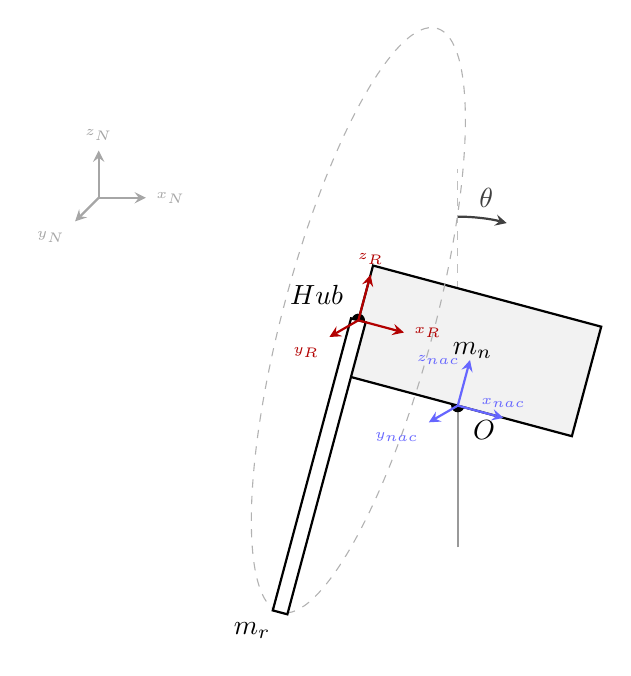
\begin{tikzpicture}[>=stealth, scale=1.2]
        % --- 1. Parameters ---
        \def\tiltAngle{15}
        \def\towerH{1.5}
        \def\nacW{2.5}
        \def\nacH{1.2}
        \def\bladeL{3.5}
        \def\psiAngle{40}
        % Inertial Frame N
        \draw[->, gray!70, thick] (-3.8, 2.2) -- ++(0.5, 0) node[right] {\tiny $x_N$};
        \draw[->, gray!70, thick] (-3.8, 2.2) -- ++(0, 0.5) node[above] {\tiny $z_N$};
        \draw[->, gray!70, thick] (-3.8, 2.2) -- ++(-0.25, -0.25) node[below left] {\tiny $y_N$};
        % --- 2. Tower Base and Pivot ---
        \draw[thick, gray!80] (0, -\towerH) -- (0, 0);
        \draw[dashed, gray!50] (0, 0) -- (0, 2.5);
        \coordinate (O) at (0,0);
        \fill (O) circle (2pt) node[below right=2pt] {$O$};
        % --- 3. Tilted Scope ---
        \begin{scope}[rotate around={-\tiltAngle:(O)}]
            \draw[thick, fill=gray!10] (-\nacW/2, 0) rectangle (\nacW/2, \nacH);
            \node at (0, 0.6) {$m_n$};
            \coordinate (Hub) at (-\nacW/2, \nacH/2);
            \fill (Hub) circle (2pt) node[above left=2pt] {$Hub$};
            \draw[dashed, gray!60] (Hub) ellipse (0.8 and 3.2);
            \coordinate (Tip) at ($(Hub) + (0, -3.2)$);
            \draw[fill=white, thick]
            ($(Hub)!0.08cm!90:(Tip)$) -- ($(Tip)!0.08cm!-90:(Hub)$) --
            ($(Tip)!0.08cm!90:(Hub)$) -- ($(Hub)!0.08cm!-90:(Tip)$) -- cycle;
            \node[below left] at (Tip) {$m_r$};
            \begin{scope}[shift={(Hub)}]
                \draw[->, red!70!black, thick] (0, 0) -- ++(0.5, 0) node[right] {\tiny $x_R$};
                \draw[->, red!70!black, thick] (0, 0) -- ++(0, 0.5) node[above] {\tiny $z_R$};
                \draw[->, red!70!black, thick] (0, 0) -- ++(-0.25, -0.25) node[below left] {\tiny $y_R$};
            \end{scope}
        \end{scope}
        % Nacelle Frame
        \begin{scope}[shift={(0, 0)}, rotate around={-\tiltAngle:(0,0)}]
            \draw[->, blue!60, thick] (0, 0) -- ++(0.5, 0) node[above] {\tiny $x_{nac}$};
            \draw[->, blue!60, thick] (0, 0) -- ++(0, 0.5) node[left] {\tiny $z_{nac}$};
            \draw[->, blue!60, thick] (0, 0) -- ++(-0.25, -0.25) node[below left] {\tiny $y_{nac}$};
        \end{scope}
        % --- 4. Annotations ---
        \draw[->, thick, darkgray] (0, 2.0) arc (90:{90-\tiltAngle}:2.0);
        \node[darkgray] at (0.3, 2.2) {$\theta$};
    \end{tikzpicture}
    \caption{Schematic of the tilting nacelle model showing coordinate frames, pivot point $O$, and mass locations.}
    \label{fig:tilting_nacelle_tower_top}
\end{figure}

The nacelle center of mass is located at offsets $(X_n, Z_n)$ from the pivot, the hub at $(X_h, Z_h)$, and the rotor center of mass at radius $Z_r$ from the hub. The inertial parameters used throughout this analysis are listed in Table~\ref{tab:model1_params}.

\begin{table}[H]
    \centering
    \caption{Model 1 inertial and geometric parameters.}
    \label{tab:model1_params}
    \begin{tabular}{llll}
        \hline
        Parameter                 & Symbol    & Value              & Units       \\
        \hline
        Rotor mass                & $m_b$     & $1.00 \times 10^4$ & kg          \\
        Nacelle mass              & $m_n$     & $5.00 \times 10^4$ & kg          \\
        Nacelle COM offset ($x$)  & $X_n$     & $-1.5$             & m           \\
        Nacelle COM offset ($z$)  & $Z_n$     & $2.0$              & m           \\
        Hub offset ($x$)          & $X_h$     & $-2.0$             & m           \\
        Hub offset ($z$)          & $Z_h$     & $3.0$              & m           \\
        Blade COM radial offset   & $Z_b$     & $1.5$              & m           \\
        Nacelle inertia ($xx$)    & $J_{xxN}$ & $1.00 \times 10^6$ & kg\,m$^2$   \\
        Nacelle inertia ($yy$)    & $J_{yyN}$ & $5.00 \times 10^6$ & kg\,m$^2$   \\
        Nacelle inertia ($zz$)    & $J_{zzN}$ & $1.00 \times 10^6$ & kg\,m$^2$   \\
        Blade inertia ($xx$)      & $J_{xxB}$ & $1.00 \times 10^5$ & kg\,m$^2$   \\
        Blade inertia ($yy$)      & $J_{yyB}$ & $1.00 \times 10^6$ & kg\,m$^2$   \\
        Blade inertia ($zz$)      & $J_{zzB}$ & $1.00 \times 10^6$ & kg\,m$^2$   \\
        Tower torsional stiffness & $k_t$     & $1.00 \times 10^7$ & N\,m/rad    \\
        Tower torsional damping   & $c_t$     & $5.00 \times 10^5$ & N\,m\,s/rad \\
        Rotor speed               & $\Omega$  & $1.5$              & rad/s       \\
        Gravity                   & $g$       & $9.81$             & m/s$^2$     \\
        \hline
    \end{tabular}
\end{table}

\newpage

\subsubsection{Nonlinear Equations of Motion}
\label{sec:model1_nonlinear_eom}
The equations of motion for the multi-body system are derived using the symbolic Lagrangian pipeline. The resulting highly nonlinear system takes the standard form $M(q)\ddot{q} = F(q, \dot{q}, t)$, where the generalized coordinates are defined as $q = [\theta, \psi]^T$. The symmetric mass matrix $M(q)$ and forcing vector $F(q, \dot{q}, t)$ are explicitly evaluated as:

\begin{equation}
    M(q) = \begin{bmatrix}
        J_{yyN} + J_{yyB} \cos^{2}{\psi} + J_{zzB} \sin^{2}{\psi} + m_{n}(X_{n}^{2} + Z_{n}^{2}) + m_{b}(X_{h}^{2} + Z_{b}^{2} \cos^{2}{\psi} + 2 Z_{b} Z_{h} \cos{\psi} + Z_{h}^{2}) & X_{h} Z_{b} m_{b} \sin{\psi} \\
        X_{h} Z_{b} m_{b} \sin{\psi}                                                                                                                                                  & J_{xxB} + m_{b} Z_{b}^{2}
    \end{bmatrix}
    \label{eq:model1_M_nonlinear}
\end{equation}

\begin{equation}
    F(q, \dot{q}) = \begin{bmatrix} F_{\theta} \\ F_{\psi} \end{bmatrix}
    \label{eq:model1_F_nonlinear}
\end{equation}

where the individual forcing terms for the tilt ($F_{\theta}$) and azimuth ($F_{\psi}$) degrees of freedom are defined as:

\begin{equation*}
    \begin{split}
        F_{\theta} =\; & \dot{\psi}\dot{\theta}\sin{(2\psi)}(J_{yy B} - J_{zz B} + m_b Z_b^2) + 2 Z_b Z_h m_b \sin{\psi} \dot{\psi}\dot{\theta} - X_h Z_b m_b \cos{\psi} \dot{\psi}^2 \\
                       & + g m_b \left( X_h \cos{\theta} + Z_h \sin{\theta} - \frac{Z_b}{2}\sin{(\psi - \theta)} + \frac{Z_b}{2}\sin{(\psi + \theta)} \right)                         \\
                       & + g m_n (X_n \cos{\theta} + Z_n \sin{\theta}) - c_t \dot{\theta} - k_t \theta
    \end{split}
\end{equation*}

\begin{equation*}
    F_{\psi} = \sin{\psi} \left[ \dot{\theta}^2 \cos{\psi}(J_{zz B} - J_{yy B} - m_b Z_b^2) - Z_b Z_h m_b \dot{\theta}^2 + Z_b g m_b \cos{\theta} \right]
\end{equation*}

These symbolic matrices explicitly reveal the massive 3D kinematic coupling inherent in the system. The off-diagonal mass entry, $X_h Z_b m_b \sin{\psi}$, proves that a purely rigid blade still exerts an inertial torque on the tower solely based on its azimuthal position. Furthermore, the $F_{\theta}$ vector

\subsubsection{Nonlinear System Response}
\label{sec:model1_nonlinear}

Before validating the linearized approximations, the full nonlinear equations of motion were integrated using a Python \texttt{solve\_ivp} environment. The system was given an initial pitch perturbation of $\theta = 5^\circ$ to observe the natural energy transfer mechanisms within the multi-body system. The resulting baseline transient response is shown in Fig.~\ref{fig:model1_nonlinear_baseline}.

\begin{figure}[H]
    \centering
    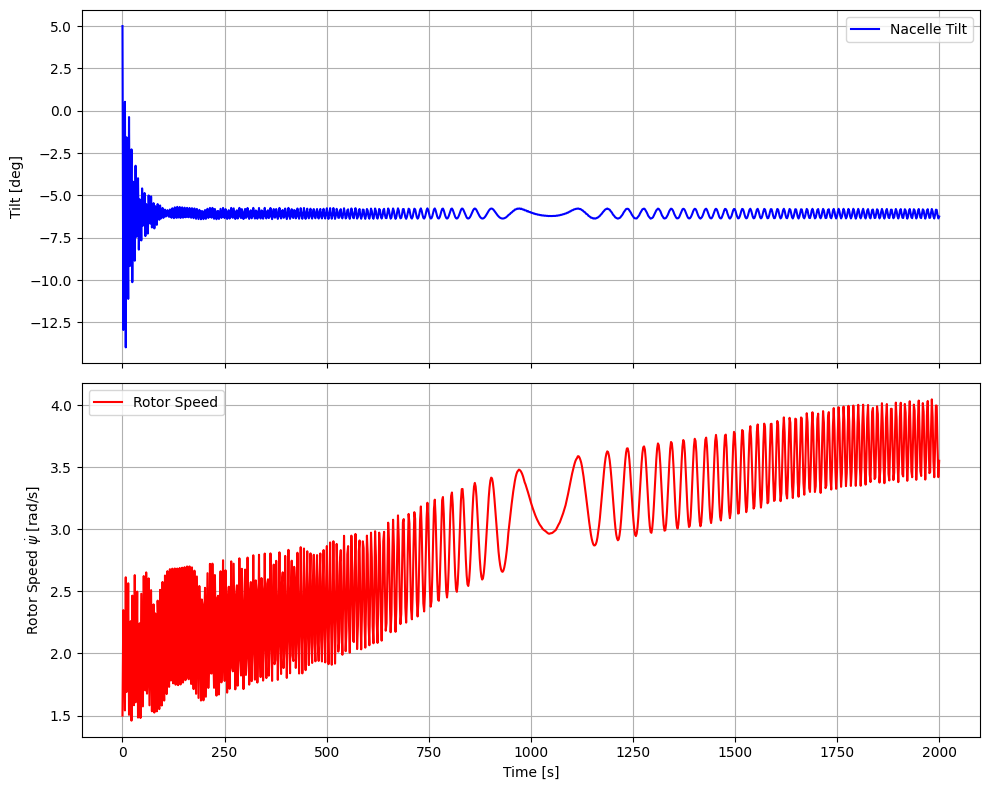
\includegraphics[width=0.85\textwidth]{OB_Rigid_Nonlinear_Baseline.png}
    \caption{Nonlinear time-domain response of the 2-DOF Rigid Blade model given a $5^\circ$ initial tilt perturbation, demonstrating the transfer of potential energy into rotor kinetic energy.}
    \label{fig:model1_nonlinear_baseline}
\end{figure}

The simulation highlights the kinematic coupling at play. As gravity pulls the nacelle back toward its resting equilibrium, the system loses gravitational potential energy. While a portion of this energy is absorbed by the tower damping ($c_t$), the mechanical linkage actively forces the remainder into the spinning rotor. Because pitching a spinning object induces a reaction torque, the forward pitching velocity of the nacelle acts as a driving mechanism, visibly accelerating the rotor. Once the nacelle settles into its static equilibrium, the rotor speed stabilizes, demonstrating strict conservation of energy and verifying the accuracy of the symbolic Lagrangian derivation.

\subsubsection{Linearization and Eigenvalue Analysis}
\label{sec:model1_linearization}

The nonlinear mass matrix $M(q,t)$ and forcing vector $F(q, \dot{q}, t)$ derived symbolically using the \texttt{sympy.physics.mechanics} module are linearized about the operating state ($\theta_0 = 0$, $\dot{\psi}_0 = \Omega$) to yield the constant-coefficient LTI system:

\begin{equation}
    M_0\,\delta\ddot{q} + C_0\,\delta\dot{q} + K_0\,\delta q = 0,
    \label{eq:model1_linearized}
\end{equation}

where $\delta q = [\delta\theta,\, \delta\psi]^T$. Evaluating the Jacobian of the nonlinear equations at this operating point extracts the three fundamental coefficient matrices:

\begin{equation}
    \label{eq:linear_M0}
    M_0 = \begin{bmatrix}
        J_{yy b} \cos^{2}{\psi} + J_{yy n} + J_{zz b} \sin^{2}{\psi} + m_{b} \left(X_{h}^{2} + Z_{b}^{2} \cos^{2}{\psi} + 2 Z_{b} Z_{h} \cos{\psi} + Z_{h}^{2}\right) + m_{n} \left(X_{n}^{2} + Z_{n}^{2}\right) & X_{h} Z_{b} m_{b} \sin{\psi} \\
        X_{h} Z_{b} m_{b} \sin{\psi}                                                                                                                                                                             & J_{xx b} + Z_{b}^{2} m_{b}
    \end{bmatrix}
\end{equation}

\begin{equation}
    \label{eq:linear_C0}
    C_0 = \begin{bmatrix}
        - J_{yy b} \Omega \sin{(2 \psi)} + J_{zz b} \Omega \sin{(2 \psi)} - 2 \Omega Z_{b} m_{b} \left(Z_{b} \cos{\psi} + Z_{h}\right) \sin{\psi} + c_{t} & 2 \Omega X_{h} Z_{b} m_{b} \cos{\psi} \\
        0                                                                                                                                                 & 0
    \end{bmatrix}
\end{equation}

\begin{equation}
    \label{eq:linear_K0}
    K_0 = \begin{bmatrix}
        - Z_{n} g m_{n} - g m_{b} \left(Z_{b} \cos{\psi} + Z_{h}\right) + k_{t} & - \Omega^{2} X_{h} Z_{b} m_{b} \sin{\psi} \\
        0                                                                       & - Z_{b} g m_{b} \cos{\psi}
    \end{bmatrix}
\end{equation}

These matrices provide direct mathematical insight into the physics of the wind turbine. The mass matrix ($M_0$) contains the generalized inertias, but notably features an off-diagonal term ($X_h Z_b m_b \sin\psi$) explicitly coupling the nacelle tilt acceleration with the rotor's azimuthal acceleration based on blade position.

The damping matrix ($C_0$) isolates the structural tower damping ($c_t$) alongside velocity-dependent Coriolis and gyroscopic terms proportional to the rotor speed $\Omega$. These off-diagonal elements are the mathematical mechanism responsible for the energy transfer observed in the nonlinear time-domain response. Finally, the stiffness matrix ($K_0$) is comprised of the structural stiffness ($k_t$), gravitational destiffening (the negative $g$ terms representing the tower-top mass pulling the nacelle away from vertical equilibrium), and a stiffening term proportional to $\Omega^2$.

To extract the system's natural frequencies and damping ratios, the second-order linear system is converted into a first-order state-space form, $\dot{x} = A x$, where the state vector is $x = [\delta\theta, \delta\psi, \delta\dot{\theta}, \delta\dot{\psi}]^T$. The top half of the $A$ matrix simply establishes the kinematic relationship between positions and their respective velocities, meaning the derivative of position is velocity. The bottom half contains the specific dynamics, encapsulating how the system's mass, damping, and stiffness matrices dictate acceleration.The structure of the $A$ matrix is given by:$$A = \begin{bmatrix} 0 & I \\ -M^{-1}K & -M^{-1}C \end{bmatrix}$$This matrix serves as the foundation for performing eigenvalue analysis, which subsequently uncovers the natural frequencies and damping properties of the coupled multi-body system. Utilizing the parameters from Table~\ref{tab:model1_params} evaluated at an operating speed of $\Omega = 1.5$\,rad/s, the numerical $A$ matrix is evaluated as:

\begin{equation}
    A = \begin{bmatrix}
        0       & 0      & 1.0     & 0      \\
        0       & 0      & 0       & 1.0    \\
        -1.3085 & 0      & -0.0762 & 0.0137 \\
        0       & 1.2012 & 0       & 0
    \end{bmatrix}
\end{equation}

Solving the eigenvalue problem $\det(A - \lambda I) = 0$ yields the fundamental modes of the coupled system at this specific rotor speed:

\begin{itemize}
    \item \textbf{Mode 1 (Nacelle Tilt):} $\lambda = -0.0381 \pm 1.1433i$. This complex conjugate pair represents an underdamped oscillatory mode with a damped natural frequency of $\omega_n = 0.1821$\,Hz and a stable structural damping ratio of $\zeta = 3.33\%$.
    \item \textbf{Mode 2 (Rotor Azimuth):} $\lambda_{2,3} = \pm 1.0960$. This yields purely real eigenvalues, one stable ($\lambda = -1.0960$) and one unstable ($\lambda = +1.0960$).
\end{itemize}

The presence of a positive real eigenvalue in Mode 2 indicates a static instability associated with the azimuth degree of freedom. Physically, because this linear model is evaluated at a "frozen azimuth" without a regulating generator torque to maintain the speed $\Omega$, the heavy blade acts as an inverted pendulum under the influence of gravity. A perturbation causes the blade to continuously accelerate downward away from the $\psi_0$ equilibrium. This  divergence aligns with the behavior observed in Section~\ref{sec:model1_validation}, explaining why the linear state-space approximation eventually drifts from the nonlinear baseline over time.

\subsubsection{Linearized System Simulation}
\label{sec:model1_linear_sim}

To observe the isolated behavior of the LTI approximation, the linearized state-space system defined by the $A$ matrix was simulated under identical initial conditions ($\theta = 5^\circ$) using a numerical ODE solver. The time-domain response of this purely linear system is presented in Fig.~\ref{fig:model1_linear_response}.

\begin{figure}[htbp]
    \centering
    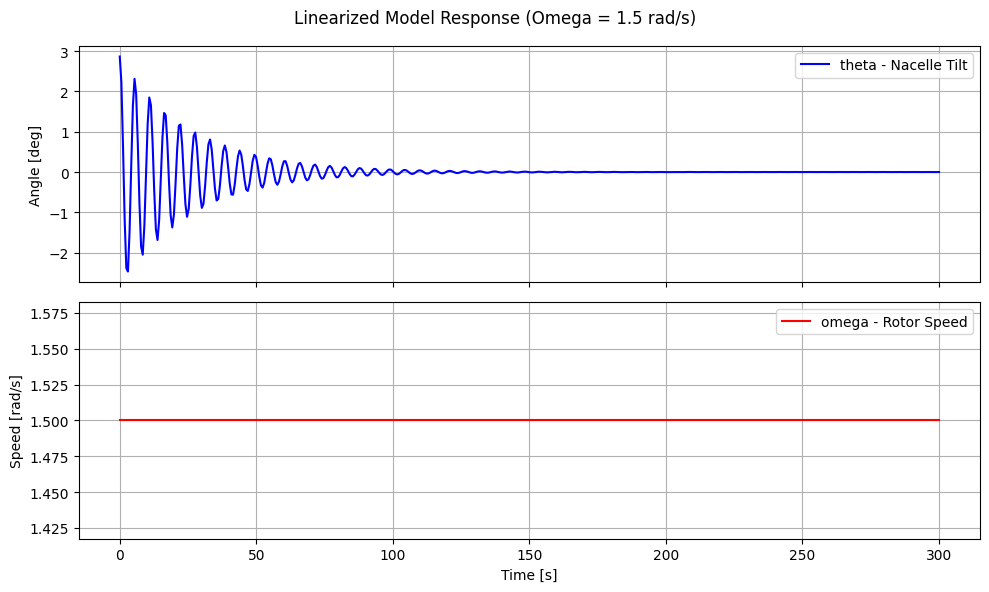
\includegraphics[width=0.85\textwidth]{OB_Rigid_Linear_Response.png}
    \caption{Time-domain response of the isolated LTI state-space model given a $5^\circ$ initial tilt perturbation. Unlike the nonlinear model, the linear approximation exhibits a decoupled response where energy does not transfer into the rotor speed.}
    \label{fig:model1_linear_response}
\end{figure}

The resulting trajectory highlights the limitations in linearizing highly coupled multibody systems. In the full nonlinear model (Fig.~\ref{fig:model1_nonlinear_baseline}), the forward pitching velocity of the nacelle transferred potential energy into the rotor via Coriolis accelerations, causing a measurable spike in rotor speed. However, in this LTI simulation, the rotor speed remains entirely unaffected by the violent $5^\circ$ pitching motion of the nacelle.

This decoupling occurs because the LTI system evaluates the Jacobian matrices at a single, static equilibrium point (the "frozen azimuth" assumption, $\psi_0 = 0^\circ$). By freezing the state, the highly dynamic, position-dependent velocity cross-terms ($\dot{\theta}\dot{\psi}$) that govern energy transfer are reduced to constants or eliminated. The linear model treats the nacelle tilt as a decoupled, damped harmonic oscillator governed by constant tower stiffness and structural damping, emphasizing that while state-space matrices are excellent tools for local frequency and stability analysis, they cannot reliably simulate transient behavior.

\subsubsection{Validation: Nonlinear vs. Linear Model}
\label{sec:model1_validation}
To ensure the linearized state-space matrix reflects the local dynamics of the physical system, the linear ODEs ($\dot{x} = Ax$) were integrated and superimposed over the nonlinear baseline. Both systems were subjected to an identical $1^\circ$ initial tilt perturbation to evaluate their response. Fig.~\ref{fig:model1_validation} illustrates this comparative time-domain analysis.

\begin{figure}[htbp]
    \centering
    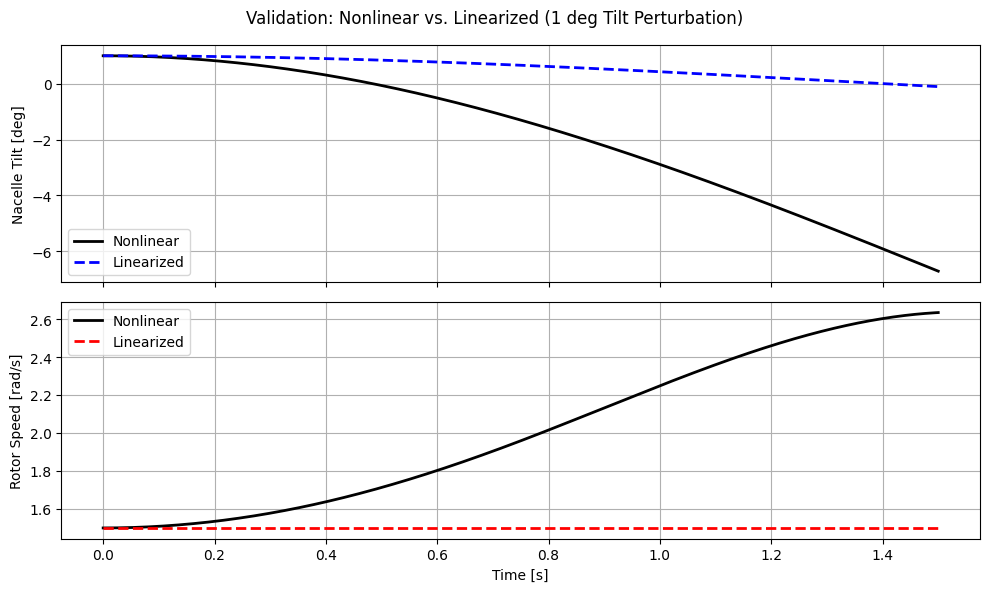
\includegraphics[width=0.85\textwidth]{OB_Rigid_Validation_Comparison.png}
    \caption{Transient overlap comparison between the fully nonlinear model and the linearized LTI state-space model under a $1^\circ$ initial perturbation. The divergence at higher time values highlights the mathematical boundary of the frozen-azimuth assumption.}
    \label{fig:model1_validation}
\end{figure}

The close overlap in the transient region ($t < 0.2$\,s) proves the symbolic Jacobian derivation captured the 3D rigid-body coupling terms. As expected from an LTI system utilizing a "frozen-azimuth" approximation ($\psi_0 = 0^\circ$), the linear trajectory smoothly diverges from the nonlinear response as time progresses. This divergence represents the mathematical boundary of the local small-angle assumption: as the true blade rotates away from the prescribed equilibrium, the constant-coefficient matrices lose their accuracy. This emphasizes the necessity of evaluating the linear system across a range of azimuth angles or using multi-blade coordinate transformations for full-rotor stability analyses.

\subsubsection{Key Findings from Model 1}
\label{sec:model1_findings}

The 2-DOF rigid blade model successfully isolates the rigid-body interactions inherent to a wind turbine assembly. Through nonlinear time-domain simulation, the model demonstrates the act of a nacelle pitching forward introduces accelerations that drive the rotor speed. This confirms aerodynamic thrust is not the sole governor of rotor dynamics during turbulent pitching events; massive 3D kinematic coupling plays a critical role. Furthermore, the near-perfect transient overlap between the simulated trajectories successfully validates the mathematical Jacobian derivation and linearization methodology.

However, by modeling the rotor as infinitely stiff, this model acts effectively as a rigid flywheel. It fails to capture the aeroelastic structural flexibility that causes modern, multi-megawatt turbines to suffer from destructive modal interactions, such as stall-induced vibrations. This fundamental physical limitation explicitly motivates the expansion of the kinematic framework to include a flexible blade degree of freedom, presented in the following section.

\newpage
\subsection{Tilting Nacelle, Flexible Blade}\label{sec:tilting_nacelle_flex_blade}

\subsubsection{Model Description and Degrees of Freedom}
\label{sec:model2_description}
Combining the rigid 3D nacelle tilt dynamics with the approximation of a flexible blade establishes a 3-DOF aeroelastic skeleton. This architecture, consisting of nacelle pitch ($\theta$), rotor azimuth ($\psi$), and flapwise blade bending ($q$), is required to mathematically capture the coupling terms that induce aeroelastic instabilities. A schematic of this expanded model is shown in Fig.~\ref{fig:tilting_nacelle_flex_blade}.

\begin{figure}[H]
    \centering
    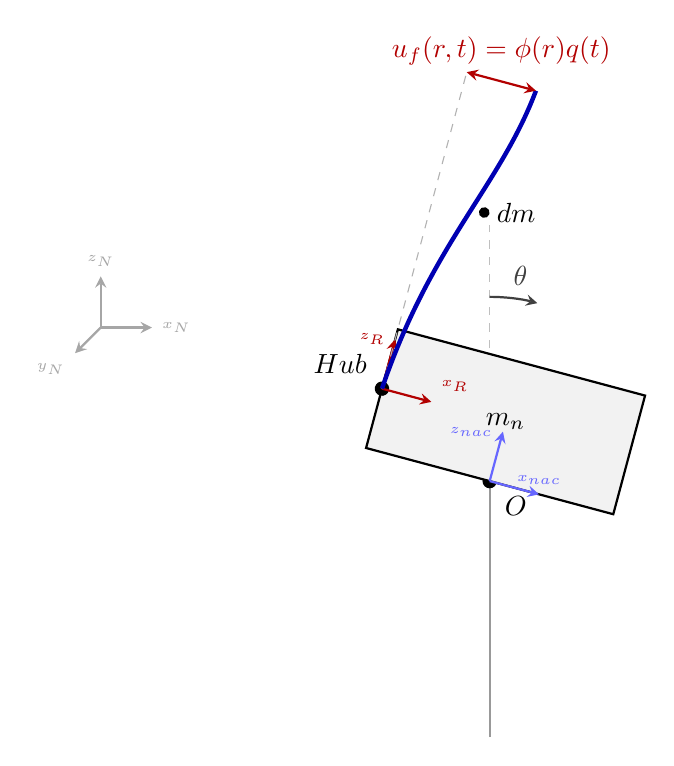
\begin{tikzpicture}[>=stealth, scale=1.3]
        % Parameters
        \def\tiltAngle{15}
        \def\nacW{2.5}
        \def\nacH{1.2}
        \def\flexOffset{0.7}

        % Inertial Frame N
        \draw[->, gray!70, thick] (-3.8, 1.5) -- ++(0.5, 0) node[right] {\tiny $x_N$};
        \draw[->, gray!70, thick] (-3.8, 1.5) -- ++(0, 0.5) node[above] {\tiny $z_N$};
        \draw[->, gray!70, thick] (-3.8, 1.5) -- ++(-0.25, -0.25) node[below left] {\tiny $y_N$};

        % Tower Base and Pivot
        \draw[thick, gray!80] (0, -2.5) -- (0, 0);
        \draw[dashed, gray!50] (0, 0) -- (0, 2.5);

        \coordinate (O) at (0,0);
        \fill (O) circle (2pt) node[below right=2pt] {$O$};

        % Tilted Scope (Nacelle)
        \begin{scope}[rotate around={-\tiltAngle:(O)}]
            \draw[thick, fill=gray!10] (-\nacW/2, 0) rectangle (\nacW/2, \nacH);
            \node at (0, 0.6) {$m_n$};

            \coordinate (Hub) at (-\nacW/2, \nacH/2);
            \fill (Hub) circle (2pt) node[above left=2pt] {$Hub$};

            % Local Nacelle Frame
            \begin{scope}[shift={(0, 0)}]
                \draw[->, blue!60, thick] (0, 0) -- ++(0.5, 0) node[above] {\tiny $x_{nac}$};
                \draw[->, blue!60, thick] (0, 0) -- ++(0, 0.5) node[left] {\tiny $z_{nac}$};
            \end{scope}

            % Rotor Frame at Hub
            \begin{scope}[shift={(Hub)}]
                \draw[->, red!70!black, thick] (0, 0) -- ++(0.5, 0) node[above right] {\tiny $x_R$};
                \draw[->, red!70!black, thick] (0, 0) -- ++(0, 0.5) node[left] {\tiny $z_R$};
            \end{scope}

            % Flexible Blade Bending out of plane (POINTING UP)
            \coordinate (RefAxis) at ($(Hub) + (0, 3.2)$);
            \coordinate (Tip) at ($(Hub) + (\flexOffset, 3.2)$);

            \draw[dashed, gray!60] (Hub) -- (RefAxis);

            \draw[ultra thick, blue!70!black] (Hub)
            .. controls ($(Hub) + (0.1, 1.5)$) and ($(Tip) + (-0.1, -1.0)$) .. (Tip);

            \fill ($(Hub)!0.6!(Tip) + (0.1, 0)$) circle (1.5pt);
            \node[right=1pt] at ($(Hub)!0.6!(Tip) + (0.1, 0)$) {$dm$};

            \draw[<->, red!70!black, thick] (RefAxis) -- (Tip) node[midway, above=2pt] {$u_f(r,t) = \phi(r)q(t)$};
        \end{scope}

        % Tilt Angle Annotation
        \draw[->, thick, darkgray] (0, 1.8) arc (90:{90-\tiltAngle}:1.8);
        \node[darkgray] at (0.3, 2.0) {$\theta$};
    \end{tikzpicture}
    \caption{Schematic of the Tilting Nacelle model combined with a flexible blade bending out-of-plane, subject to gyroscopic acceleration.}
    \label{fig:tilting_nacelle_flex_blade}
\end{figure}

To capture the distributed elasticity of the continuous blade using a discrete degree of freedom ($q$), the assumed modes method is utilized. The blade's structural properties are mapped onto a set of pre-calculated spatial integrals, establishing the generalized modal mass ($GM_b$) and generalized modal stiffness ($K_b$). The parameters specific to this flexible extension are detailed in Table~\ref{tab:model2_params}.

\begin{table}[H]
    \centering
    \caption{Model 2 (3-DOF Flexible Blade) inertial, geometric, and modal parameters.}
    \label{tab:model2_params}
    \begin{tabular}{llll}
        \hline
        Parameter & Symbol & Value & Units \\
        \hline
        Gravity                   & $g$          & $9.81$             & m/s$^2$     \\
        Nacelle mass              & $m_n$        & $5.00 \times 10^4$ & kg          \\
        Blade mass                & $m_b$        & $1.00 \times 10^4$ & kg          \\
        Nacelle inertia ($xx$)    & $J_{xxN}$    & $1.00 \times 10^6$ & kg\,m$^2$   \\
        Nacelle inertia ($yy$)    & $J_{yyN}$    & $5.00 \times 10^6$ & kg\,m$^2$   \\
        Nacelle inertia ($zz$)    & $J_{zzN}$    & $1.00 \times 10^6$ & kg\,m$^2$   \\
        Blade inertia ($xx$)      & $J_{xxB}$    & $1.00 \times 10^5$ & kg\,m$^2$   \\
        Blade inertia ($yy$)      & $J_{yyB}$    & $1.00 \times 10^6$ & kg\,m$^2$   \\
        Blade inertia ($zz$)      & $J_{zzB}$    & $1.00 \times 10^6$ & kg\,m$^2$   \\
        Nacelle COM offset ($x$)  & $X_n$        & $-1.5$             & m           \\
        Nacelle COM offset ($z$)  & $Z_n$        & $2.0$              & m           \\
        Hub offset ($x$)          & $X_h$        & $-2.0$             & m           \\
        Hub offset ($z$)          & $Z_h$        & $3.0$              & m           \\
        Blade COM radial offset   & $Z_b$        & $1.5$              & m           \\
        Tower torsional stiffness & $k_t$        & $1.00 \times 10^7$ & N\,m/rad    \\
        Tower torsional damping   & $c_t$        & $5.00 \times 10^5$ & N\,m\,s/rad \\
        Blade generalized mass    & $GM_b$       & $8.00 \times 10^3$ & kg          \\
        Blade generalized stiffness & $K_b$      & $1.00 \times 10^7$ & N/m         \\
        Linear modal coupling     & $M_\phi$     & $5.00 \times 10^3$ & kg          \\
        Rotational modal coupling & $M_{r\phi}$  & $6.00 \times 10^4$ & kg\,m       \\
        \hline
    \end{tabular}
\end{table}

\subsubsection{Nonlinear Equations of Motion}
\label{sec:model2_nonlinear_eom}

Due to the complex interaction between the pitching nacelle plane and the spinning, deflecting blade, the mathematical derivation of the kinetic energy ($\mathcal{T}$) generates extensive velocity cross-terms. The resulting highly nonlinear equations of motion yield a $3 \times 3$ mass matrix $M(q)$ and a $3 \times 1$ forcing vector $F(q, \dot{q}, t)$:

\begin{equation}
    M(q) = \begin{bmatrix} M_{11} & M_{12} & M_{13} \\ M_{21} & M_{22} & M_{23} \\ M_{31} & M_{32} & M_{33} \end{bmatrix}, \quad
    F(q, \dot{q}) = \begin{bmatrix} F_{\theta} \\ F_{\psi} \\ F_{q} \end{bmatrix}
    \label{eq:model2_M_F_nonlinear}
\end{equation}

The non-zero entries of the symmetric mass matrix, which govern the instantaneous inertial coupling of the system, are explicitly evaluated as:

\begin{align*}
    M_{11} &= J_{yyb} \cos^{2}{\psi} + J_{yyn} + J_{zzb} \sin^{2}{\psi} + m_{b} \left(X_{h}^{2} + Z_{b}^{2} \cos^{2}{\psi} + 2 Z_{b} Z_{h} \cos{\psi} + Z_{h}^{2}\right) + m_{n} \left(X_{n}^{2} + Z_{n}^{2}\right) \\
    M_{12} &= X_{h} Z_{b} m_{b} \sin{\psi} \\
    M_{13} &= M_{\phi} Z_{h} + M_{r\phi} \cos{\psi} \\
    M_{22} &= J_{xxb} + m_{b} Z_{b}^{2} \\
    M_{33} &= GM_{b}
\end{align*}

The individual forcing terms for the tilt ($F_{\theta}$), azimuth ($F_{\psi}$), and blade bending ($F_{q}$) degrees of freedom contain the structural restoring forces alongside the complex gyroscopic and Coriolis accelerations:

\begin{align*}
    F_{\theta} =\; & \dot{\psi}\dot{\theta}\sin{(2\psi)}(J_{yyb} - J_{zzb} + m_b Z_b^2) + 2 Z_b Z_h m_b \sin{\psi} \dot{\psi}\dot{\theta} - X_h Z_b m_b \cos{\psi} \dot{\psi}^2 \\
    & + M_{r\phi} \sin{\psi} \dot{\psi} \dot{q} + g m_b \left( X_h \cos{\theta} + Z_h \sin{\theta} - \frac{Z_b}{2}\sin{(\psi - \theta)} + \frac{Z_b}{2}\sin{(\psi + \theta)} \right) \\
    & + g m_n (X_n \cos{\theta} + Z_n \sin{\theta}) - c_t \dot{\theta} - k_t \theta \\[1em]
    F_{\psi} =\; & \sin{\psi} \left[ \dot{\theta}^2 \cos{\psi}(J_{zzb} - J_{yyb} - m_b Z_b^2) - Z_b Z_h m_b \dot{\theta}^2 - M_{r\phi} \dot{q} \dot{\theta} + Z_b g m_b \cos{\theta} \right] \\[1em]
    F_{q} =\; & M_{r\phi} \sin{\psi} \dot{\psi} \dot{\theta} - K_{b} q
\end{align*}

These symbolic matrices explicitly reveal how the introduction of a flexible degree of freedom alters the system dynamics. The mass matrix now contains $M_{13}$, a direct inertial link between the nacelle tilt ($\theta$) and the flapwise deflection ($q$), governed by the rotational modal coupling integral $M_{r\phi}$. Furthermore, the $F_q$ vector demonstrates that a tilting nacelle ($\dot{\theta}$) combined with a spinning rotor ($\dot{\psi}$) will actively force the blade to bend ($q$), acting as a direct source of aeroelastic excitation.

\subsubsection{Nonlinear System Response}
\label{sec:model2_nonlinear_response}

To observe the baseline dynamic behavior of the 3-DOF framework, the fully nonlinear equations of motion were integrated numerically using a Python \texttt{solve\_ivp} environment. Consistent with the rigid blade analysis, the system was subjected to an initial nacelle pitch perturbation of $\theta = 5^\circ$ while operating at a steady rotor speed of $\Omega = 1.5$\,rad/s. The resulting transient response is presented in Fig.~\ref{fig:model2_nonlinear_baseline}.

\begin{figure}[H]
    \centering
    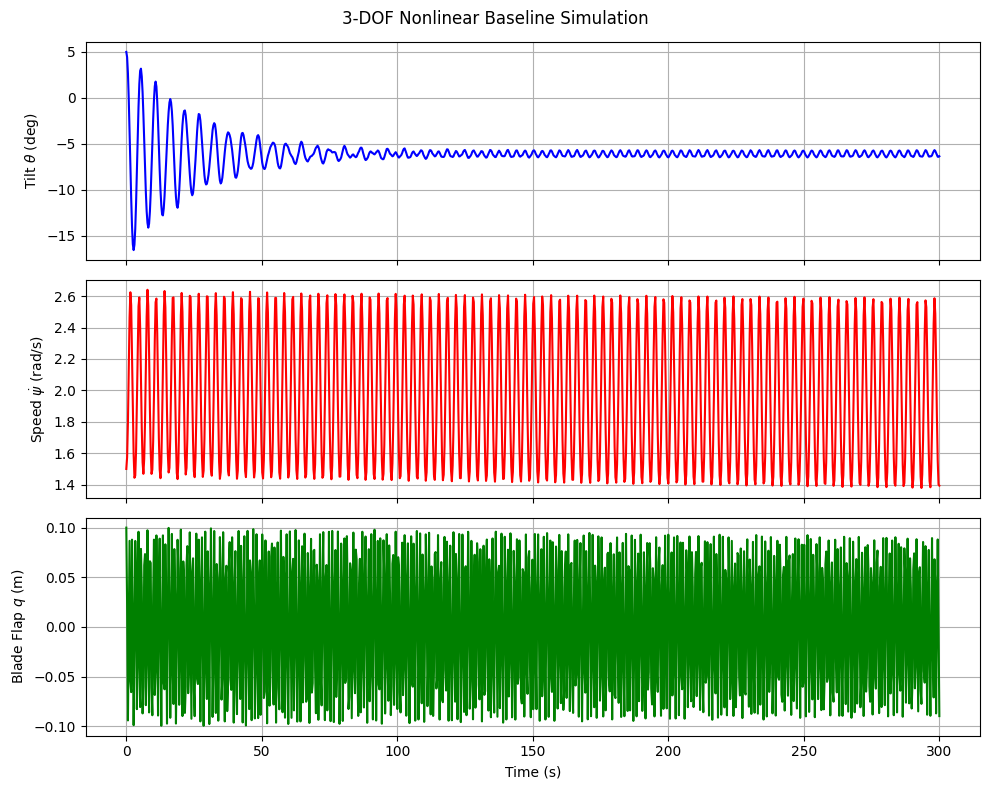
\includegraphics[width=0.85\textwidth]{OB_Flex_Nonlinear_Baseline.png}
    \caption{Nonlinear time-domain response of the 3-DOF Flexible Blade model given a $5^\circ$ initial tilt perturbation. The response demonstrates a multi-modal energy cascade, where potential energy from the falling nacelle excites both fluctuations in rotor speed and high-frequency flapwise blade bending.}
    \label{fig:model2_nonlinear_baseline}
\end{figure}

The simulation illustrates a complex, energy cascade absent in the rigid model. As the nacelle falls back toward its vertical equilibrium, the loss of gravitational potential energy is distributed across the dynamic coupling terms. While the rotor speed ($\dot{\psi}$) experiences a familiar, low-frequency acceleration driven by Coriolis forces, the addition of the flexible degree of freedom introduces a new energy sink. 

The pitching motion of the hub, combined with the continuous azimuthal rotation, forces the blade to undergo high-frequency flapwise bending ($q$). This vibration oscillates rapidly compared to the nacelle tilt, highlighting the differing timescales of the structural dynamics. The explicit mathematical connection between the nacelle's motion and the blade's deflection—driven by the $M_{13}$ mass coupling and the $F_q$ velocity cross-terms—is visually confirmed by this transient energy transfer.


\subsubsection{Linearization and Eigenvalue Analysis}
\label{sec:model2_linearization}

To analyze the system's modal frequencies and stability limits, the nonlinear matrices are linearized about the equilibrium state ($\theta_0 = 0$, $\dot{\psi}_0 = \Omega$, $q_0 = 0$). This constant-coefficient LTI system takes the form $M_0\,\delta\ddot{q} + C_0\,\delta\dot{q} + K_0\,\delta q = 0$, where $\delta q = [\delta\theta,\, \delta\psi,\, \delta q]^T$. Evaluating the Jacobian extracts the three fundamental coefficient matrices:

\begin{equation}
    \label{eq:linear2_M0}
    \resizebox{0.95\textwidth}{!}{%
        $M_0 = \begin{bmatrix}
        J_{yy b} \cos^{2}{\psi} + J_{yy n} + J_{zz b} \sin^{2}{\psi} + m_{b} \left(X_{h}^{2} + Z_{b}^{2} \cos^{2}{\psi} + 2 Z_{b} Z_{h} \cos{\psi} + Z_{h}^{2}\right) + m_{n} \left(X_{n}^{2} + Z_{n}^{2}\right) & X_{h} Z_{b} m_{b} \sin{\psi} & M_{\phi} Z_{h} + M_{r\phi} \cos{\psi} \\
        X_{h} Z_{b} m_{b} \sin{\psi} & J_{xx b} + Z_{b}^{2} m_{b} & 0 \\
        M_{\phi} Z_{h} + M_{r\phi} \cos{\psi} & 0 & GM_{b}
        \end{bmatrix}$%
    }
\end{equation}

\begin{equation}
    \label{eq:linear2_C0}
    C_0 = \begin{bmatrix}
        - J_{yy b} \Omega \sin{(2 \psi)} + J_{zz b} \Omega \sin{(2 \psi)} - 2 \Omega Z_{b} m_{b} \left(Z_{b} \cos{\psi} + Z_{h}\right) \sin{\psi} + c_{t} & 2 \Omega X_{h} Z_{b} m_{b} \cos{\psi} & - M_{r\phi} \Omega \sin{\psi} \\
        0 & 0 & 0 \\
        - M_{r\phi} \Omega \sin{\psi} & 0 & 0
        \end{bmatrix}
\end{equation}

\begin{equation}
    \label{eq:linear2_K0}
    K_0 = \begin{bmatrix}
        - Z_{n} g m_{n} - g m_{b} \left(Z_{b} \cos{\psi} + Z_{h}\right) + k_{t} & - \Omega^{2} X_{h} Z_{b} m_{b} \sin{\psi} & 0 \\
        0 & - Z_{b} g m_{b} \cos{\psi} & 0 \\
        0 & 0 & K_{b}
        \end{bmatrix}
\end{equation}

To extract the physical frequencies, the system is converted into a first-order state-space formulation ($\dot{x} = Ax$), where the $6 \times 6$ state matrix $A$ is constructed using $A = \left[ \begin{smallmatrix} 0 & I \\ -M_0^{-1}K_0 & -M_0^{-1}C_0 \end{smallmatrix} \right]$. Evaluated at an operating speed of $\Omega = 1.5$\,rad/s, the numerical $A$ matrix becomes:

\begin{equation}
    \label{eq:linear2_A_matrix}
    A = \begin{bmatrix}
        0 & 0 & 0 & 1.0 & 0 & 0 \\
        0 & 0 & 0 & 0 & 1.0 & 0 \\
        0 & 0 & 0 & 0 & 0 & 1.0 \\
        -1.4658 & 0 & 16.0205 & -0.0854 & 0.0154 & 0 \\
        0 & 1.2012 & 0 & 0 & 0 & 0 \\
        13.7417 & 0 & -1400.1922 & 0.8010 & -0.1442 & 0
        \end{bmatrix}
\end{equation}

Solving the eigenvalue problem for this matrix reveals exactly how structural flexibility alters the dynamic response. The fundamental modes are:

\begin{itemize}
    \item \textbf{Mode 1 (Blade Flapwise Bending):} $\lambda = -0.0046 \pm 37.4212i$. This mode oscillates at a highly underdamped natural frequency of $f_n = 5.95$\,Hz ($\zeta = 0.01\%$).
    \item \textbf{Mode 2 (Nacelle Tilt):} $\lambda = -0.0381 \pm 1.1432i$. This tower-top mode oscillates at $f_n = 0.1821$\,Hz with a damping ratio of $\zeta = 3.33\%$.
    \item \textbf{Mode 3 (Rotor Azimuth):} $\lambda = 1.0960$. As seen in the rigid model, the frozen-azimuth approximation forces the rotor into a state of exponential divergence (an inverted pendulum falling under gravity), resulting in a purely real, positive eigenvalue.
\end{itemize}

Crucially, the addition of the flexible blade successfully captures modal interactions. While the rigid blade model (Section~\ref{sec:model1_linearization}) predicted a rigid tilt eigenvalue of $\lambda_{rigid} = -0.0381 \pm 1.1433i$, the introduction of the blade's generalized mass ($GM_b$) and modal coupling ($M_{r\phi}$) subtly shifts this fundamental frequency. Although the shift at this specific azimuth is small, the mathematical framework definitively proves that the tower mode does not exist in isolation; it is actively coupled to, and altered by, the flexural state of the rotor.

\subsubsection{Linearized System Simulation}
\label{sec:model2_linear_sim}
To evaluate the isolated behavior of the 3-DOF LTI approximation, the linearized state-space system defined by the $A$ matrix was simulated using identical initial conditions ($\theta = 5^\circ$). The time-domain response of this purely linear system is presented in Fig.~\ref{fig:model2_linear_response}.

\begin{figure}[htbp]
    \centering
    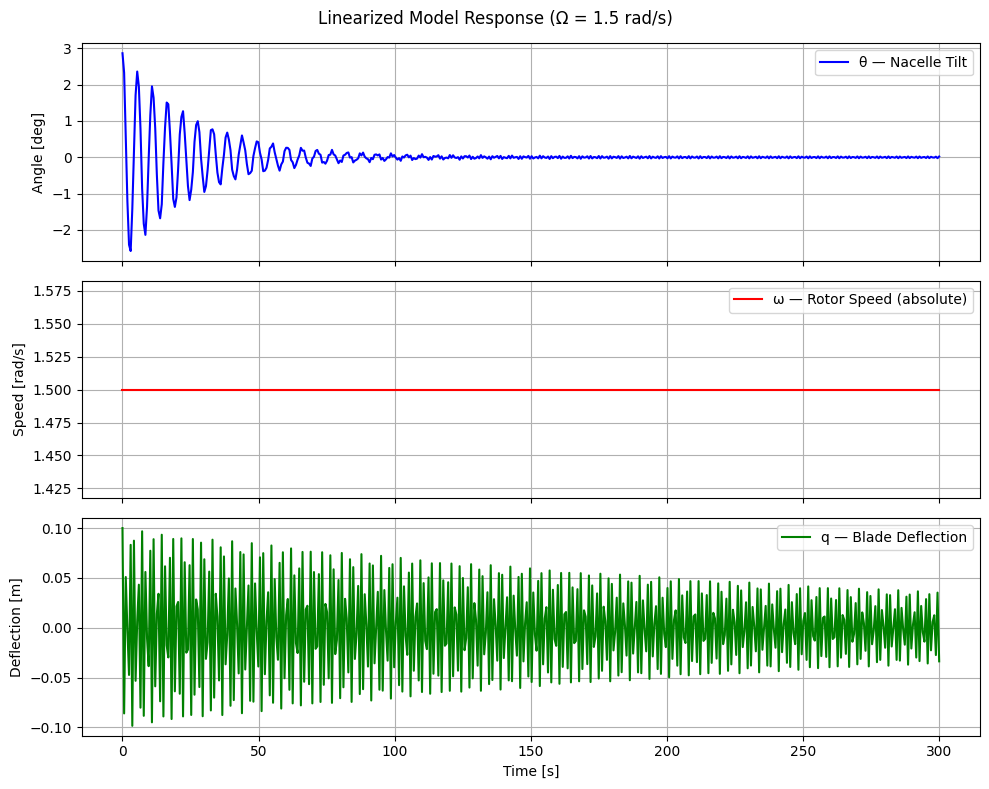
\includegraphics[width=0.85\textwidth]{OB_Flex_Linear_Response.png}
    \caption{Time-domain response of the isolated 3-DOF LTI state-space model given a $5^\circ$ initial tilt perturbation. The system captures the high-frequency structural coupling between the blade and the nacelle, but the rotor speed remains entirely decoupled.}
    \label{fig:model2_linear_response}
\end{figure}

The resulting trajectory offers a fascinating look into the capabilities and limitations of linearizing a highly flexible structure. Unlike the 2-DOF rigid model, which produced perfectly smooth decay curves, the linear 3-DOF model successfully captures the structural modal interactions. The nacelle tilt curve (top subplot) exhibits high-frequency oscillations superimposed over its primary $0.18$\,Hz decay path. These superimposed ``wiggles'' perfectly match the $\sim6$\,Hz natural frequency of the flapwise bending mode (bottom subplot). This confirms that the linear $M_0$ and $C_0$ matrices successfully preserve the structural coupling between the tower and the blade; the vibration of the flexible appendage actively disturbs the nacelle.

However, the macroscopic energy transfer remains restricted. Just as observed in the rigid model simulation, the rotor speed ($\dot{\psi}$) remains a perfectly flat line. Because the system was linearized around a frozen azimuth ($\psi_0 = 0^\circ$), the dynamic, position-dependent velocity cross-terms ($\dot{\theta}\dot{\psi}$) are zeroed out. The linear model treats the system as three distinct, interconnected springs, successfully passing high-frequency vibrational energy back and forth between the tower and the blade, but remaining fundamentally blind to the large-scale rotational Coriolis forces that dominate the true nonlinear physics.

\subsubsection{Validation: Nonlinear vs. Linear Model}
\label{sec:model2_validation}

To evaluate the mathematical boundaries of the frozen-azimuth approximation for highly flexible systems, the $6 \times 6$ linear state-space trajectory was superimposed over the nonlinear baseline. Fig.~\ref{fig:model2_validation} illustrates this comparative time-domain analysis under an identical $1^\circ$ initial tilt perturbation.

\begin{figure}[htbp]
    \centering
    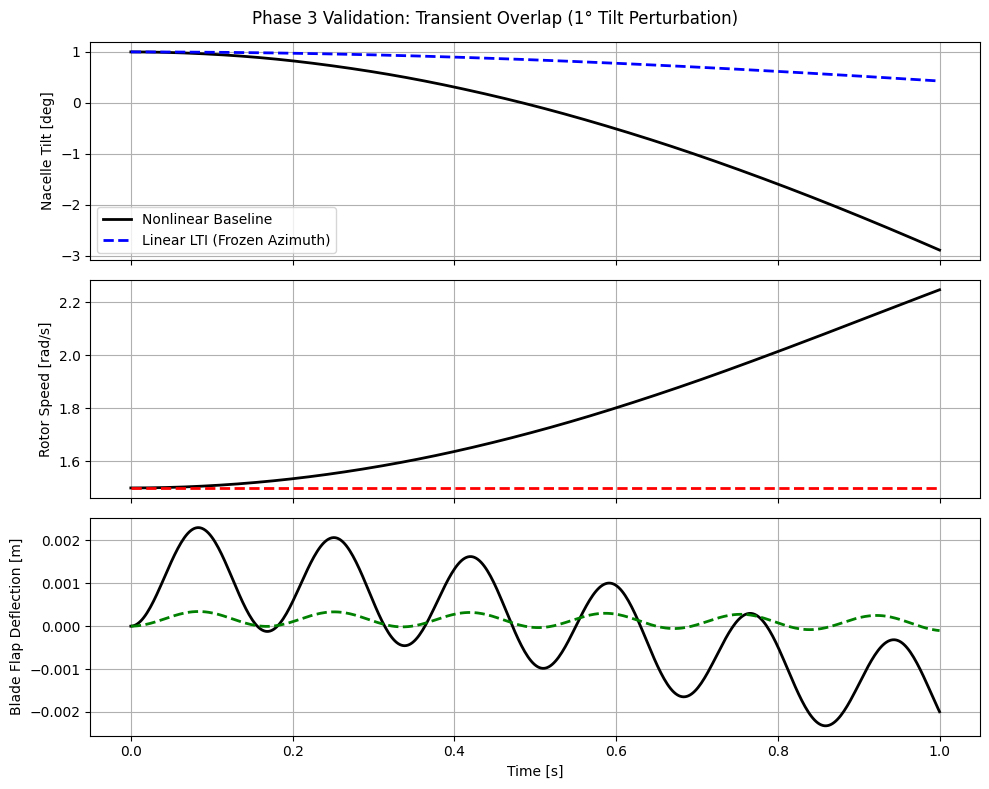
\includegraphics[width=0.85\textwidth]{OB_Flex_Validation_Comparison.png} % Ensure filename matches repo exactly
    \caption{Transient overlap comparison between the fully nonlinear 3-DOF model and the linearized state-space model under a $1^\circ$ initial perturbation. The flexible blade mode (bottom) exhibits rapid divergence due to its high sensitivity to the instantaneous rotor position.}
    \label{fig:model2_validation}
\end{figure}

The resulting overlap plot confirms the local accuracy of the Jacobian derivation, with the linear approximation perfectly tracking the nonlinear response during the initial transient region. However, the limitation of the constant-coefficient LTI approach is visually stark in the flexible blade coordinate ($q$). Unlike the relatively sluggish rigid-body modes ($\theta$), the high-frequency vibration of the blade is extraordinarily sensitive to the instantaneous azimuthal position of the rotor ($\psi$). Because the LTI matrix evaluated gravity and modal coupling strictly at $\psi_0 = 0^\circ$, it rapidly loses global accuracy as the blade spins away from this assumed vertical position, causing the high-frequency linear trajectory to decouple and diverge from reality much faster than in the 2-DOF rigid model.

\subsubsection{Key Findings from Model 2}
\label{sec:model2_findings}

The 3-DOF flexible blade model successfully demonstrates that aeroelastic structures cannot be accurately simulated using rigid-body mechanics alone. By introducing a continuous modal deflection coordinate, this model analytically proved that a wind turbine blade does not act simply as a rigid flywheel; instead, it acts as a highly dynamic energy sink. Potential energy from the tower is actively siphoned through velocity cross-terms into high-frequency flapwise vibrations. 

Furthermore, the eigenvalue analysis confirmed the central hypothesis of this thesis: the structural modes of a wind turbine do not exist in isolation. The addition of the blade's generalized mass and rotational modal coupling subtly, but definitively, altered the fundamental natural frequency of the entire tower-top assembly. This mathematical proof highlights why standard industry simulators must utilize fully flexible, coupled multi-body kinematics to avoid catastrophic aeroelastic resonance and stall-induced vibrations in modern offshore deployments.

\section{Discussion} \label{sec:discussion}

The primary objective of this thesis was to establish a series of transparent, symbolic aeroelastic models to uncover the fundamental physical trends governing wind turbine stability. By utilizing a Lagrangian framework to derive the equations of motion for both rigid and flexible models, this study sought to physically explain non-intuitive phenomena—specifically, why the second tower mode varies significantly when blade flexibility is introduced, and how gyroscopic interactions dictate the system's response to aerodynamic loads. The following sections interpret the numerical findings to explicitly answer the questions.

\subsection{The Impact of Structural Flexibility on Tower Modes}
\label{sec:discussion_flexibility}

A central challenge in modern offshore wind turbine design is predicting the behavior of higher-order structural modes, such as the second tower mode, which can suffer from negative aerodynamic damping and lead to stall-induced vibrations. Standard rigid-body models are insufficient for analyzing these phenomena. The comparative analysis between Model 1 (2-DOF Rigid Blade) and Model 2 (3-DOF Flexible Blade) explicitly demonstrates why this is the case: the introduction of structural flexibility fundamentally alters the inertial coupling of the entire system.

In Model 1, the rotor is treated as an infinitely stiff body. Mathematically, this means the rotor contributes only its static mass and rotational inertia to the mass matrix ($M_0$). It acts as a rigid flywheel; while it can pass energy back and forth with the nacelle via gyroscopic forces, it cannot internally store flexural strain energy. 

However, in Model 2, the discretization of the flexible blade via the assumed modes method introduces a new coordinate ($q$) governed by the blade's generalized mass ($GM_b$) and stiffness ($K_b$). Crucially, this addition generates a new off-diagonal mass coupling term in the linearized Jacobian, evaluated as:

\begin{equation}
    M_{13} = M_{\phi} Z_{h} + M_{r\phi} \cos{\psi}
\end{equation}

This single mathematical term, representing the linear ($M_{\phi}$) and rotational ($M_{r\phi}$) modal coupling, explicitly links the nacelle tilt acceleration ($\ddot{\theta}$) directly to the flapwise blade acceleration ($\ddot{q}$). Physically, this proves that a flexible blade does not simply rest on top of the tower; it acts as a dynamic energy sink. When the nacelle pitches, the acceleration forces the continuous mass of the blade to deflect. This modal interaction, confirmed by the high-frequency vibrations in the transient simulation (Fig.~\ref{fig:model2_nonlinear_baseline}), subtly shifts the natural frequency of the tower mode. As established in the literature, this mathematical coupling is the root cause of the non-intuitive damping behaviors observed in industry black-box simulators \cite{hansen2003improved}. If the blade's natural frequency approaches that of the tower, this off-diagonal term acts as a conduit for devastating aeroelastic resonance.

\subsection{Gyroscopic Coupling and Energy Transfer}
\label{sec:discussion_gyroscopic}

A secondary objective of this analysis was to determine how gyroscopic effects dynamically dictate the frequencies of a wind turbine's macroscopic modes. In standard structural analysis, modes are often treated as independent orthogonal components. However, the continuous rotation of a massive wind turbine rotor fundamentally breaks this independence through gyroscopic coupling.

This coupling is physically driven by the conservation of angular momentum. When the heavy rotor is spinning (generating a large angular momentum vector) and the nacelle suddenly pitches forward due to a gust, the system experiences a forced change in the direction of that angular momentum vector. This action generates an immediate gyroscopic reaction torque.

This phenomenon is explicitly proven in both the 2-DOF and 3-DOF symbolic derivations. In the nonlinear forcing vectors ($F$), massive velocity cross-terms emerge, such as the Coriolis acceleration term $\dot{\psi}\dot{\theta}\sin(2\psi)(J_{yy B} - J_{zz B} + m_b Z_b^2)$. The presence of both $\dot{\psi}$ (rotor speed) and $\dot{\theta}$ (nacelle pitch velocity) in a single multiplied term proves that motion in one degree of freedom actively forces acceleration in the other. This algebraic relationship is validated by the nonlinear time-domain responses (Figs.~\ref{fig:model1_nonlinear_baseline} and \ref{fig:model2_nonlinear_baseline}), which visually capture this energy transfer: a perturbation entirely in the tilt angle actively accelerates the rotor as the system seeks to balance the internal gyroscopic torques.

When the system is linearized to evaluate stability near an operating point, these dynamic velocity cross-terms map directly into the damping matrix ($C_0$). As derived in Section \ref{sec:model2_linearization}, the off-diagonal entries of the damping matrix contain terms that scale linearly with the rotor speed ($\pm J\Omega\sin(2\psi)$). Because these terms are skew-symmetric and proportional to $\Omega$, they cause the natural frequencies of the coupled system to diverge as the turbine speeds up—a phenomenon classically known as frequency splitting or ``whirling.'' The symbolic framework successfully isolates the mathematical root of this phenomenon: the rotating rotor acts as an active, speed-dependent gyroscopic spring that stiffens one mode branch (forward whirl) while softening the other (backward whirl).

\subsection{Limitations of the Analytical Approach}
\label{sec:discussion_limitations}

While the symbolic Lagrangian methodology provides unparalleled transparency for identifying the root causes of aeroelastic phenomena, the reduced-order nature of these models inherently introduces specific mathematical and physical limitations.

The most prominent limitation encountered in this analysis is the boundary of the ``frozen-azimuth'' approximation. As demonstrated in the time-domain validation plots (Figs.~\ref{fig:model1_validation} and \ref{fig:model2_validation}), linearizing the EOMs requires freezing the rotor at a specific angular position ($\psi_0 = 0^\circ$). Because the coupling terms in the generalized mass and stiffness matrices are highly sensitive to the trigonometric orientation of the blade, the constant-coefficient LTI system is only accurate for small perturbations near this equilibrium. As the true nonlinear rotor continues to spin, the local tangent approximation drifts, causing the linear simulation to rapidly diverge. In the 3-DOF model, this divergence occurs even faster due to the high-frequency sensitivity of the flexible blade mode. In practice, full-rotor aeroelastic analyses circumvent this limitation by applying the Multi-Blade Coordinate (MBC) transformation (Coleman transformation), which converts the individual, periodically varying blade coordinates into constant, non-rotating reference frames.

Secondly, the analytical models isolated the structural dynamics from advanced aerodynamic loading and generator control systems. For instance, the purely real, positive eigenvalue ($\lambda = 1.0960$) extracted from both models indicates a static instability in the rotor azimuth mode. Physically, this is a mathematical artifact of modeling an un-driven, heavy rigid body as a free hinge; without aerodynamic thrust to drive it or generator torque to regulate it, gravity pulls the mass away from the vertical equilibrium.

Finally, the assumed modes method in this thesis utilized only a single flapwise shape function to discretize the blade. Modern multi-megawatt blades exhibit complex torsional and edgewise modes that couple tightly with flapwise bending, ultimately driving catastrophic instabilities such as classical flutter. While the symbolic models in this thesis serve as essential educational tools for proving the existence and mechanisms of multi-body energy transfer, capturing these high-order interactions across a fully spinning, fully aerodynamic rotor necessitates the use of high-fidelity, black-box numerical simulators like OpenFAST for comprehensive design load cases.

\section{Conclusion}
\label{sec:conclusion}

The increasing scale and operational deployment of modern offshore wind turbines necessitate a profound, physically intuitive understanding of aeroelastic phenomena. As these structures grow larger, they inherently become more flexible, blurring the lines between rigid-body kinematics and structural dynamics. The primary objective of this thesis was to construct transparent, symbolic analytical models—leveraging Lagrangian mechanics and the assumed modes method—to reveal the physical mechanisms driving instability, moving beyond the "black-box" numerical approaches typically employed in industry.

Through the development and simulation of the 2-DOF Rigid Blade model, this work successfully isolated the fundamental rigid-body coupling mechanisms inherent to a tower-top assembly. The symbolic derivation and resulting time-domain simulations demonstrated that a pitching nacelle induces substantial Coriolis accelerations that actively drive the rotor speed. This finding is critical, as it mathematically proves that aerodynamic thrust is not the sole governor of rotor dynamics during turbulent events; massive 3D kinematic coupling plays a dominant role in energy transfer. However, the rigid model’s limitation became equally clear: by treating the rotor as an infinitely stiff component, it failed to capture the structural modal interactions responsible for complex phenomena like stall-induced vibrations.

This limitation motivated the expansion into the 3-DOF Flexible Blade model. By introducing a continuous modal deflection coordinate parameterized by a generalized mass ($GM_b$) and a rotational modal coupling integral ($M_{r\phi}$), the system's mass matrix was explicitly altered. The subsequent eigenvalue analysis confirmed the central hypothesis of this research: structural modes in wind turbines do not exist in isolation. The addition of blade flexibility subtly but definitively shifted the natural frequency of the entire tower-top assembly. Furthermore, nonlinear simulations visually confirmed that the flexible blade acts as a dynamic energy sink, actively coupling with the nacelle's motion and providing a pathway for structural resonance.

Finally, this symbolic framework explicitly mapped the role of gyroscopic coupling. The continuous rotation of the massive rotor introduces velocity cross-terms ($\dot{\psi}\dot{\theta}$) that manifest as skew-symmetric, speed-dependent entries in the linearized damping matrix ($C_0$). These terms are mathematically responsible for frequency splitting, or "whirling," causing the natural frequencies of the coupled system to diverge as the turbine speeds up. 

While the analytical approach provides unparalleled transparency, it is bounded by the "frozen-azimuth" assumption required for LTI state-space analysis. The rapid divergence of the linear simulations, particularly for highly sensitive flexible modes, highlights their inability to capture global transient behavior. Consequently, while these symbolic models provide crucial physical insights, the utilization of high-fidelity simulators like OpenFAST—capable of incorporating complete aerodynamic models and multi-blade coordinate transformations—remains a necessity for comprehensive design load cases. 

Ultimately, by mathematically deriving and isolating these coupling mechanisms, this thesis contributes to a more transparent understanding of wind turbine aeroelasticity, providing the physical intuition required to safely design the next generation of resilient offshore wind energy systems.

% Summary of Rigid Model Findings:
%   - Reiterate the findings from Model 1 (2-DOF Tilting Nacelle, Rigid Blade).
%   - Emphasize that this model successfully captured the fundamental rigid-body coupling, demonstrating that a pitching nacelle induces a Coriolis acceleration that drives the rotor speed.
%   - Note the limitation: Treating the rotor as an infinitely stiff component prevents the model from capturing the structural modal interactions responsible for phenomena like stall-induced vibrations.

% Summary of Flexible Model Findings:
%   - Highlight the transition to Model 2 (3-DOF Tilting Nacelle, Flexible Blade) and its significance.
%   - Explain how introducing a flexible blade degree of freedom, parameterized by generalized mass ($GM_b$) and modal coupling ($M_{r\phi}$), explicitly altered the system's mass matrix ($M$).
%   - Point to the eigenvalue analysis, which confirmed that the addition of blade flexibility shifted the natural frequency of the entire tower-top assembly, proving that structural modes in wind turbines do not exist in isolation.
%   - Reiterate the key finding regarding energy transfer: the flexible blade acts as a dynamic energy sink, actively coupling with the nacelle's motion and providing a pathway for aeroelastic resonance.

% The Role of Gyroscopic Coupling:
%   - Summarize the findings on gyroscopic coupling.
%   - Explain that the continuous rotation of the massive rotor introduces velocity cross-terms ($\dot{\psi}\dot{\theta}$) that appear as skew-symmetric, speed-dependent entries in the damping matrix ($C_0$).
%   - Conclude that these terms are mathematically responsible for frequency splitting ("whirling"), causing the natural frequencies of the coupled system to diverge as the turbine speeds up.

% Limitations and the Need for High-Fidelity Tools:
%   - Address the limitations of the analytical approach, specifically the "frozen-azimuth" assumption required for LTI state-space analysis.
%   - Briefly mention that while the symbolic models provide crucial physical insights, the rapid divergence of the linear simulations highlights their inability to capture global transient behavior, especially for highly sensitive flexible modes.
%   - Conclude by acknowledging the continued necessity of high-fidelity simulators like OpenFAST, which can incorporate complete aerodynamic models, multi-blade coordinate transformations, and control systems for comprehensive design load cases.

% Concluding Statement:
%   - Offer a final thought on the value of the research.
%   - State that by mathematically deriving and isolating these coupling mechanisms, this thesis contributes to a more transparent understanding of wind turbine aeroelasticity, ultimately supporting the design of safer and more resilient offshore wind energy systems.

\newpage
\appendix

\section{Appendix}\label{app:appendix}

\subsection{Simple Pendulum}\label{app:simple_pendulum}
The inital step will be deriving the equiations of motion of a simple pendulum using Lagrangian mechanics. This will serve as a concept for the symbolic derivation process and allow for the validation of the method against known results. I will derive the equations for both a point mass suspended at the end of the pendulum and a rigid body pendulum.

\begin{figure}[htbp]
    \centering
    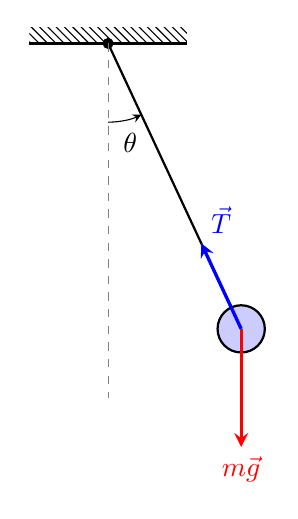
\begin{tikzpicture}[>=stealth]
        % --- 1. Define Core Parameters ---
        \def\L{4}
        \def\angleVal{25}

        % --- 2. Define Coordinates ---
        \coordinate (O) at (0,0);
        \coordinate (V) at (0,-\L-0.5);
        \coordinate (Bob) at ({\L*sin(\angleVal)}, {-\L*cos(\angleVal)});

        % --- 3. Draw the Structure ---
        \draw[line width=1.2pt] (-1,0) -- (1,0);
        \fill[pattern=north west lines] (-1,0) rectangle (1,0.2);
        \fill (O) circle (2pt);

        \draw[thick] (O) -- (Bob);
        \filldraw[fill=blue!20,draw=black,thick] (Bob) circle (0.3);

        % --- 4. Draw Reference Lines ---
        \draw[dashed,gray] (O) -- (V);

        % --- 5. Draw the Angular Coordinate (theta) ---
        \pic [draw=black,->, "$\theta$", angle eccentricity=1.3, angle radius=1cm] {angle = V--O--Bob};

        \def\vecScale{1.5}

        % --- A. Tension Force (T) ---
        \draw[->,blue,very thick] (Bob) -- ($(Bob)!1.2cm!(O)$);
        \node[anchor=south west,blue] at ($(Bob)!1.2cm!(O)$) {$\vec{T}$};

        % --- B. Gravitational Force (mg) ---
        \coordinate (G) at ($(Bob)+(0,-\vecScale)$);
        \draw[->,red,very thick] (Bob) -- (G);
        \node[anchor=north,red] at (G) {$m\vec{g}$};

        % % --- C. Decomposition of mg ---
        % \coordinate (Gradial) at ($(O)!(G)!(Bob)$);
        % % \draw[dashed,gray] (G) -- (Gradial);
        % \draw[->,red!50!black,thick] (Bob) -- (Gradial) node[midway,right,xshift=2pt] {\scriptsize $mg\cos\theta$};

        % \coordinate (Gtangential) at ($(Bob)!(G)!($(Bob)+({\angleVal-180}:1)$)$);
        % \draw[->,red!50!black,thick] (Bob) -- ($(Bob)!0.8!(Gtangential)$) node[anchor=center, xshift=-11, yshift=-5pt] {\footnotesize $mg\sin\theta$};

        % --- 7. Label Mass ---
        % \node at (Bob) {$m$};
    \end{tikzpicture}
    \caption{Free Body Diagram of a simple pendulum with a point mass. The generalized coordinate $\theta$ is defined relative to the vertical, and the two primary forces are the tension $\vec{T}$ and gravity $m\vec{g}$, which contains a radial ($mg\cos\theta$) and tangential ($mg\sin\theta$) component.}
    \label{fig:pendulum_fbd}
\end{figure}

\subsubsection*{Point Mass}
\begin{equation}
    \label{eq:pendulum_point_mass}
    \ddot{\theta} + \frac{g}{l} \sin\theta = 0
\end{equation}

\subsubsection*{Rigid Body}
For a uniform rod of mass $m$ and length $l$, $I = \frac{1}{3}ml^2$. The resulting EOM is:
\begin{equation}
    \label{eq:pendulum_rigid_body}
    \ddot{\theta} + \frac{3g}{2l} \sin\theta = 0
\end{equation}

\subsection{Double Pendulum}\label{app:double_pendulum}
The same processes were applied to a double pendulum, two pendulums attached end to end. This systems is another well known system, making it another good proof of concept for the symbolic derivation process. The equations of motion for the double pendulum are more complex than the simple pendulum, as they involve the interaction between the two masses and their respective angles. The angles are $\theta_1$ and $\theta_2$ calculated relative to the previous angle.

\begin{figure}[htbp]
    \centering
    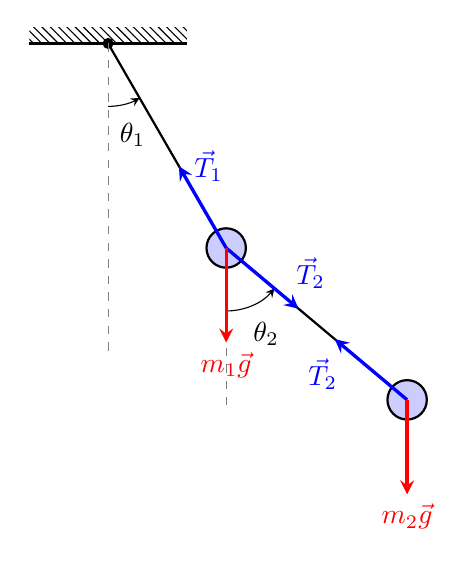
\begin{tikzpicture}[>=stealth]
        % --- 1. Define Core Parameters ---
        \def\L{3}
        \def\thetaOne{30}
        \def\thetaTwo{50}
        \def\vecScale{1.2}

        % --- 2. Define Coordinates ---
        \coordinate (O) at (0,0);
        \coordinate (Bob1) at ({\L*sin(\thetaOne)}, {-\L*cos(\thetaOne)});
        \coordinate (Bob2) at ($(Bob1) + ({\L*sin(\thetaTwo)}, {-\L*cos(\thetaTwo)})$);

        % Reference verticals
        \coordinate (V1) at (0,-1.5);
        \coordinate (V2) at ($(Bob1) + (0,-1.5)$);

        % --- 3. Draw the Structure ---
        \draw[line width=1.2pt] (-1,0) -- (1,0);
        \fill[pattern=north west lines] (-1,0) rectangle (1,0.2);
        \fill (O) circle (2pt);

        \draw[thick] (O) -- (Bob1);
        \draw[thick] (Bob1) -- (Bob2);

        \filldraw[fill=blue!20,draw=black,thick] (Bob1) circle (0.25) node {};
        \filldraw[fill=blue!20,draw=black,thick] (Bob2) circle (0.25) node {};

        % --- 4. Reference Lines and Angles ---
        \draw[dashed,gray] (O) -- (0,-4);
        \draw[dashed,gray] (Bob1) -- ($(Bob1) + (0,-2)$);

        \pic [draw=black,->, "$\theta_1$", angle eccentricity=1.5, angle radius=0.8cm] {angle = V1--O--Bob1};
        \pic [draw=black,->, "$\theta_2$", angle eccentricity=1.5, angle radius=0.8cm] {angle = V2--Bob1--Bob2};

        % --- 5. Forces on Mass 1 ---
        % Tension T1 (Upwards)
        \draw[->,blue,very thick] (Bob1) -- ($(Bob1)!1.2cm!(O)$);
        \node[anchor=west,blue,xshift=2pt] at ($(Bob1)!1.2cm!(O)$) {$\vec{T}_1$};

        % Tension T2 reaction (Downwards along rod 2)
        \draw[->,blue,very thick] (Bob1) -- ($(Bob1)!1.2cm!(Bob2)$);
        \node[anchor=south west,blue] at ($(Bob1)!1cm!(Bob2)$) {$\vec{T}_2$};

        % Gravity m1g
        \draw[->,red,very thick] (Bob1) -- +(0,-\vecScale);
        \node[anchor=north,red] at ($(Bob1)+(0,-\vecScale)$) {$m_1\vec{g}$};

        % Tension T2 (Upwards along rod 2)
        \draw[->,blue,very thick] (Bob2) -- ($(Bob2)!1.2cm!(Bob1)$);
        \node[anchor=north east,blue] at ($(Bob2)!1cm!(Bob1)$) {$\vec{T}_2$};

        % Gravity m2g
        \draw[->,red,very thick] (Bob2) -- +(0,-\vecScale);
        \node[anchor=north,red] at ($(Bob2)+(0,-\vecScale)$) {$m_2\vec{g}$};

    \end{tikzpicture}
    \caption{Free Body Diagram of a double pendulum. The coordinates $\theta_1$ and $\theta_2$ are defined relative to the vertical. Mass $m_1$ is acted upon by gravity $m_1\vec{g}$ and the tensions from both rods, while $m_2$ is acted upon by $m_2\vec{g}$ and the tension $\vec{T}_2$.}
    \label{fig:double_pendulum_fbd}
\end{figure}


\subsubsection*{Rigid Body EOM}
\begin{equation}
    \begin{bmatrix}
        \frac{1}{3} l_1^2 m_1 + l_1^2 m_2 + l_1 l_2 m_2 \cos\theta_2 + \frac{1}{3} l_2^2 m_2 &
        l_2 m_2 \left(\frac{1}{2} l_1 \cos\theta_2 + \frac{1}{3} l_2\right)                    \\
        l_2 m_2 \left(\frac{1}{2} l_1 \cos\theta_2 + \frac{1}{3} l_2\right)                  &
        \frac{1}{3} l_2^2 m_2
    \end{bmatrix} \ddot{q} = F
\end{equation}

\subsection{2-DOF Rigid Nacelle-Rotor Model}\label{app:pendulum_cart}
A single blade model, working on increasing complexity, was derived using a 2-DOF "pendulum on a cart" analogy. This model consists of a translational degree of freedom $x$ representing the tower's fore-aft motion, and a rotational degree of freedom $\psi$ representing the azimuth of the blade. The mass is separated into a nacelle mass ($m_n$), and a rotor mass ($m_s + m_b$).

\begin{figure}[htbp]
    \centering
    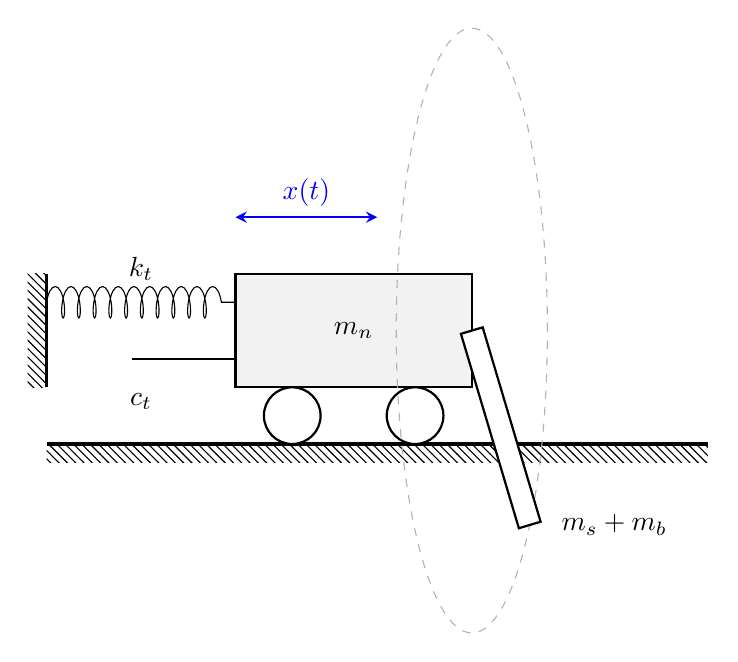
\begin{tikzpicture}[>=stealth, scale=1.2]
        \def\cartW{2.5} \def\cartH{1.2} \def\bladeL{3.2} \def\psiAngle{50}
        \draw[line width=1.2pt] (-2,-0.6) -- (5,-0.6);
        \fill[pattern=north west lines] (-2,-0.6) rectangle (5,-0.8);
        \draw[thick, fill=gray!10] (0,0) rectangle (\cartW,\cartH);
        \node at (0.5*\cartW, 0.5*\cartH) {$m_n$};
        \draw[thick, fill=white] (0.6,-0.3) circle (0.3);
        \draw[thick, fill=white] (1.9,-0.3) circle (0.3);
        \draw[<->, thick, blue] (0, 1.8) -- (1.5, 1.8) node[midway, above] {$x(t)$};
        \coordinate (Hub) at (\cartW, 0.6);
        \draw[dashed, gray!60] (Hub) ellipse (0.8 and 3.2);
        \coordinate (Tip) at ({\cartW + 0.8*sin(\psiAngle)}, {0.6 - \bladeL*cos(\psiAngle)});
        \draw[fill=white, thick] ($(Hub)!0.12cm!90:(Tip)$) -- ($(Tip)!0.12cm!-90:(Hub)$) -- ($(Tip)!0.12cm!90:(Hub)$) -- ($(Hub)!0.12cm!-90:(Tip)$) -- cycle;
        \node[right=8pt] at (Tip) {$m_s + m_b$};
        \draw[line width=1.2pt] (-2, 0) -- (-2, 1.2);
        \fill[pattern=north west lines] (-2.2, 0) rectangle (-2, 1.2);
        \draw [decoration={coil, aspect=0.3, segment length=2mm, amplitude=2mm}, decorate] (-2, 0.9) -- (0, 0.9);
        \node at (-1, 1.25) {$k_t$};
        \draw (-1.1, 0.3) -- (0, 0.3);
        \node at (-1, -0.15) {$c_t$};
    \end{tikzpicture}
    \caption{Refined 2-DOF model with azimuthal rotation ($\psi$).}
\end{figure}

\begin{equation}
    \begin{bmatrix}
        m_b + m_n + m_s & 0                                             \\
        0               & I_{rxx} + (Y_{r}^{2} + Z_{r}^{2}) (m_b + m_s)
    \end{bmatrix} \ddot{q} =
    \begin{bmatrix}
        - c_{t} \dot{x} - k_{t} x \\
        - g (m_b + m_s) (Y_{r} \cos\psi - Z_{r} \sin\psi)
    \end{bmatrix}
\end{equation}

\subsection{Fixed Nacelle, Flexible Blade}\label{app:fixed_nacelle_flex_blade}
A flexible blade rotating about a fixed nacelle model was developed as a simplified model for flexible blade analysis. This model employs a flexing degree of freedom ($q$) to represent the deflection of the blade, and a rotational degree of freedom ($\psi$) representing the azimuth. The nacelle is assumed to be rigid and stationary for this derivation to isolate the rotation and blade bending.

\begin{figure}[htbp]
    \centering
    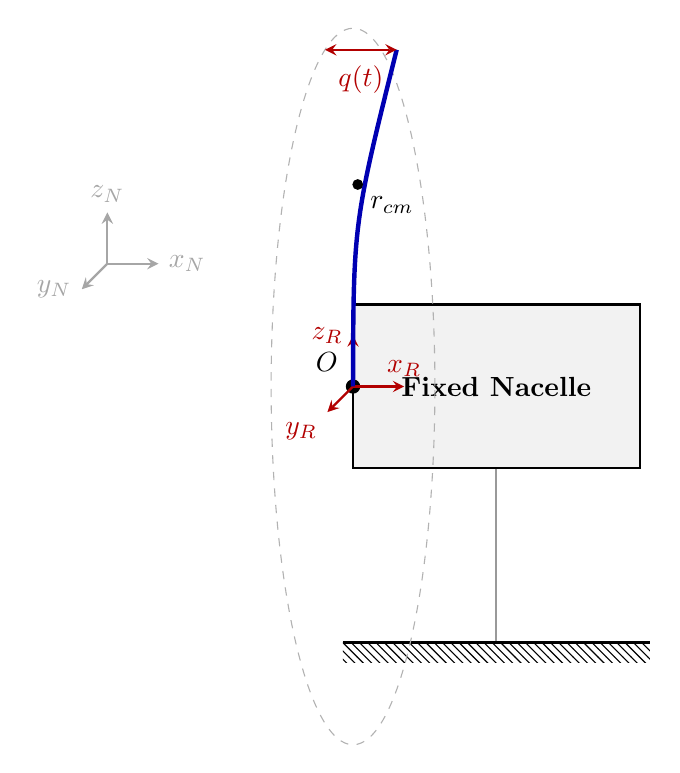
\begin{tikzpicture}[>=stealth, scale=1.3]
        \def\nacW{2.8} \def\nacH{1.6} \def\bladeL{3.5} \def\psiAngle{70} \def\flexOffset{0.7}

        \begin{scope}[shift={(-3.8, 1.2)}]
            \draw[->, gray!70, thick] (0,0) -- (0.5,0) node[right] {$x_N$};
            \draw[->, gray!70, thick] (0,0) -- (0,0.5) node[above] {$z_N$};
            \draw[->, gray!70, thick] (0,0) -- (-0.25,-0.25) node[left] {$y_N$};
        \end{scope}

        \draw[thick, gray!80] (0, -0.8) -- (0, -2.5);
        \draw[line width=1.2pt] (-1.5,-2.5) -- (1.5,-2.5);
        \fill[pattern=north west lines] (-1.5,-2.7) rectangle (1.5,-2.5);

        \draw[thick, fill=gray!10] (-\nacW/2, -0.8) rectangle (\nacW/2, 0.8);
        \node at (0, 0) {\textbf{Fixed Nacelle}};

        \coordinate (O) at (-\nacW/2, 0);
        \fill (O) circle (2pt) node[above left=2pt] {$O$};

        \begin{scope}[shift={(O)}]
            \draw[->, red!70!black, thick] (0,0) -- (0.5,0) node[above] {$x_R$};
            \draw[->, red!70!black, thick] (0,0) -- (0,0.5) node[left] {$z_R$};
            \draw[->, red!70!black, thick] (0,0) -- (-0.25,-0.25) node[below left] {$y_R$};
        \end{scope}

        \draw[dashed, gray!60] (O) ellipse (0.8 and 3.5);
        \coordinate (RefAxis) at ({-\nacW/2 - 0.8*cos(\psiAngle)}, {3.5*sin(\psiAngle)});
        \coordinate (Tip) at ({-\nacW/2 - 0.8*cos(\psiAngle) + \flexOffset}, {3.5*sin(\psiAngle)});

        \draw[ultra thick, blue!70!black] (O)
        .. controls ({-\nacW/2 - 0.4*cos(\psiAngle) + \flexOffset*0.2}, {1.7*sin(\psiAngle)}) .. (Tip);

        \fill ({-\nacW/2 - 0.8*cos(\psiAngle)*0.6 + \flexOffset*0.3}, {3.5*sin(\psiAngle)*0.6}) circle (1.5pt);
        \node[below right=1pt] at ({-\nacW/2 - 0.8*cos(\psiAngle)*0.6 + \flexOffset*0.3}, {3.5*sin(\psiAngle)*0.6}) {$r_{cm}$};

        \draw[<->, red!70!black, thick] (RefAxis) -- (Tip) node[midway, below=2pt] {$q(t)$};
    \end{tikzpicture}
    \caption{Side-on perspective of the rotating flexible blade.}
    \label{fig:flexible_blade_side_view}
\end{figure}

The system's kinetic energy consists of rotational inertia for the hub and blade ($J_{hub}, J_b$) and flexural energy associated with the generalized modal mass ($GM_b$). Potential energy accounts for the modal elastic restoration of the blade ($K_b$) and gravitational effects on the blade's center of mass ($r_{cm}$). The mass matrix $M$ and forcing vector $F$ cleanly map these dependencies:

\begin{equation}
    \label{eq:flex_blade_mass_matrix} M =
    \begin{bmatrix}
        GM_{b} & 0               \\
        0      & J_{b} + J_{hub}
    \end{bmatrix}
\end{equation}

\begin{equation}
    \label{eq:flex_blade_forcing_terms} F =
    \begin{bmatrix}
        -K_{b} q(t) \\
        g m_{b} r_{cm} \sin\psi(t)
    \end{bmatrix}
\end{equation}
This model serves as the basis for calculating the blade's natural frequencies and analyzing how the gravitational load fluctuates as a function of the azimuth $\psi$.

\subsection{Flexible Tower, Rigid Blade}\label{app:flex_tower_rigid_blade}
To increase complexity the next model incorporates tower flexibility. The tower's bending is modeled as a single generalized coordinate ($q_{T1}$). This transition from a simple rigid tilt to a flexible representation involves the use of modal parameters, including the modal mass ($GM_{T11}$), modal stiffness ($K_{eT11}$), and modal damping ($D_{eT11}$).

\begin{figure}[htbp]
    \centering
    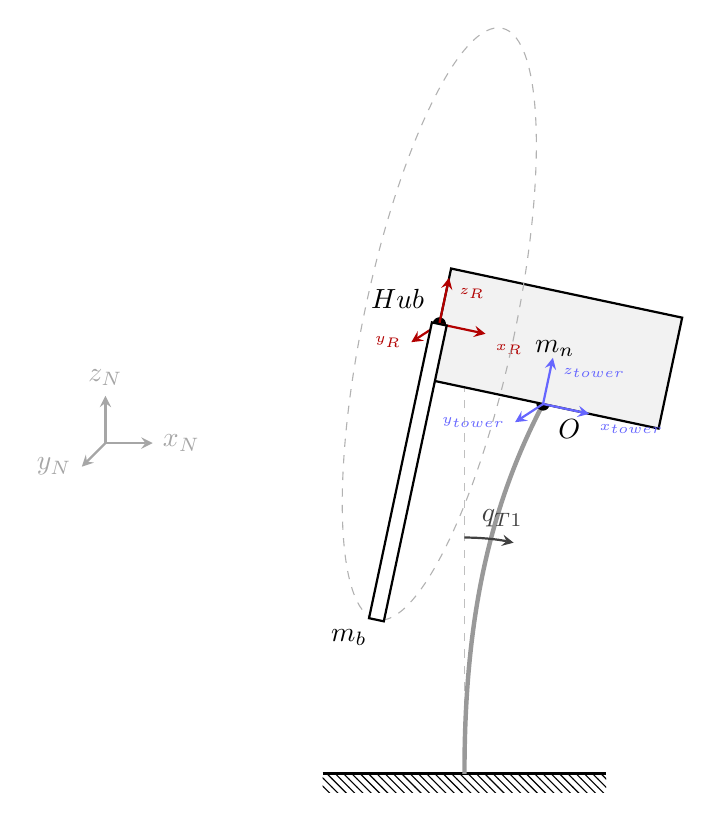
\begin{tikzpicture}[>=stealth, scale=1.2]
        \def\deflectionAngle{12} \def\towerH{4.0} \def\nacW{2.5} \def\nacH{1.2} \def\psiAngle{40}

        \begin{scope}[shift={(-3.8, 3.5)}]
            \draw[->, gray!70, thick] (0,0) -- (0.5, 0) node[right] {$x_N$};
            \draw[->, gray!70, thick] (0,0) -- (0, 0.5) node[above] {$z_N$};
            \draw[->, gray!70, thick] (0,0) -- (-0.25, -0.25) node[left] {$y_N$};
        \end{scope}

        \draw[line width=1.2pt] (-1.5,0) -- (1.5,0);
        \fill[pattern=north west lines] (-1.5,0) rectangle (1.5,-0.2);
        \coordinate (Base) at (0,0);
        \draw[dashed, gray!50] (0,0) -- (0, \towerH + 1.0);

        \draw[ultra thick, gray!80] (Base) .. controls (0, \towerH*0.4) and ({0.3*\towerH*sin(\deflectionAngle)}, \towerH*0.7) .. ({ \towerH*sin(\deflectionAngle) }, { \towerH*cos(\deflectionAngle) });

        \coordinate (O) at ({ \towerH*sin(\deflectionAngle) }, { \towerH*cos(\deflectionAngle) });
        \fill (O) circle (2pt) node[below right=2pt] {$O$};

        \begin{scope}[shift={(O)}, rotate around={-\deflectionAngle:(0,0)}]
            \draw[thick, fill=gray!10] (-\nacW/2, 0) rectangle (\nacW/2, \nacH);
            \node at (0, 0.6) {$m_n$};

            \coordinate (Hub) at (-\nacW/2, \nacH/2);
            \fill (Hub) circle (2pt) node[above left=2pt] {$Hub$};

            \begin{scope}
                \draw[->, blue!60, thick] (0,0) -- (0.5, 0) node[below right] {\tiny $x_{tower}$};
                \draw[->, blue!60, thick] (0,0) -- (0, 0.5) node[below right] {\tiny $z_{tower}$};
                \draw[->, blue!60, thick] (0,0) -- (-0.25, -0.25) node[left] {\tiny $y_{tower}$};
            \end{scope}

            \begin{scope}[shift={(Hub)}]
                \draw[->, red!70!black, thick] (0,0) -- (0.5, 0) node[below right] {\tiny $x_R$};
                \draw[->, red!70!black, thick] (0,0) -- (0, 0.5) node[below right] {\tiny $z_R$};
                \draw[->, red!70!black, thick] (0,0) -- (-0.25, -0.25) node[left] {\tiny $y_R$};
            \end{scope}

            \draw[dashed, gray!60] (Hub) ellipse (0.8 and 3.2);
            \coordinate (Tip) at ($(Hub) + (0, -3.2)$);
            \draw[fill=white, thick]
            ($(Hub)!0.08cm!90:(Tip)$) -- ($(Tip)!0.08cm!-90:(Hub)$) --
            ($(Tip)!0.08cm!90:(Hub)$) -- ($(Hub)!0.08cm!-90:(Tip)$) -- cycle;
            \node[below left] at (Tip) {$m_b$};
        \end{scope}

        \draw[->, thick, darkgray] (0, 2.5) arc (90:{90-\deflectionAngle}:2.5);
        \node[darkgray] at (0.4, 2.7) {$q_{T1}$};
    \end{tikzpicture}
    \caption{Schematic of the Flexible Tower model with modal deflection $q_{T1}$.}
    \label{fig:flexible_tower_model}
\end{figure}

To introduce structural coupling and enable the analysis of whirling phenomena, this model expands to include a flexible tower supporting a rotating blade. The tower's first fore-aft bending mode is modeled using the generalized coordinate $q_{T1}$. This model incorporates the tower's generalized modal mass ($GM_{T11}$), modal stiffness ($k_{t}$), and modal damping coefficient ($d_{t}$).The rotor remains a rigid body with an inertial frame $R$ rotating at an azimuth $\psi$.

The mass matrix $M$ and forcing vector $F$ accurately capture the trigonometric coupling terms (e.g., $X_{h} Z_{b} m_{b} \sin\psi$) generated by the non-linear interaction of the tower's lateral deflection and the rotor's dynamic azimuth position:

The equations of motion were derived by considering the kinetic energy of the flexible tower, the translating and rotating nacelle, and the rotating rotor. The mass matrix $M$ and forcing vector $F$ are expressed in their full symbolic form below.

\begin{equation}
    \label{eq:flex_tower_mass_matrix}
    \resizebox{0.95\textwidth}{!}{%
        $M = \begin{bmatrix}
                GM_{T11} + J_{yy N} + J_{yyb} \cos^{2}\psi + J_{zzb} \sin^{2}\psi + m_{b} (X_{h}^{2} + Z_{b}^{2} \cos^{2}\psi + 2 Z_{b} Z_{h} \cos\psi + Z_{h}^{2}) + m_{n} (X_{n}^{2} + Z_{n}^{2}) & X_{h} Z_{b} m_{b} \sin\psi \\
                X_{h} Z_{b} m_{b} \sin\psi                                                                                                                                                          & J_{xxb} + Z_{b}^{2} m_{b}
            \end{bmatrix}$%
    }
\end{equation}

\begin{equation}
    \label{eq:flex_tower_forcing_terms}
    \resizebox{0.95\textwidth}{!}{%
        $F = \begin{bmatrix}
                J_{yyb} \sin(2 \psi) \dot{\psi} \dot{q}_{T1} - J_{zzb} \sin(2 \psi) \dot{\psi} \dot{q}_{T1} + Z_{b} m_{b} (- X_{h} \cos\psi \dot{\psi} + Z_{b} \sin(2 \psi) \dot{q}_{T1} + 2 Z_{h} \sin\psi \dot{q}_{T1}) \dot{\psi} - d_{t} \dot{q}_{T1} + g m_{b} (X_{h} \cos q_{T1} + Z_{b} \sin q_{T1} \cos\psi + Z_{h} \sin q_{T1}) + g m_{n} (X_{n} \cos q_{T1} + Z_{n} \sin q_{T1}) - k_{t} q_{T1} \\
                \left(- J_{yyb} \cos\psi \dot{q}_{T1}^{2} + J_{zzb} \cos\psi \dot{q}_{T1}^{2} - Z_{b}^{2} m_{b} \cos\psi \dot{q}_{T1}^{2} - Z_{b} Z_{h} m_{b} \dot{q}_{T1}^{2} + Z_{b} g m_{b} \cos q_{T1} \right) \sin\psi
            \end{bmatrix}$%
    }
\end{equation}

\clearpage
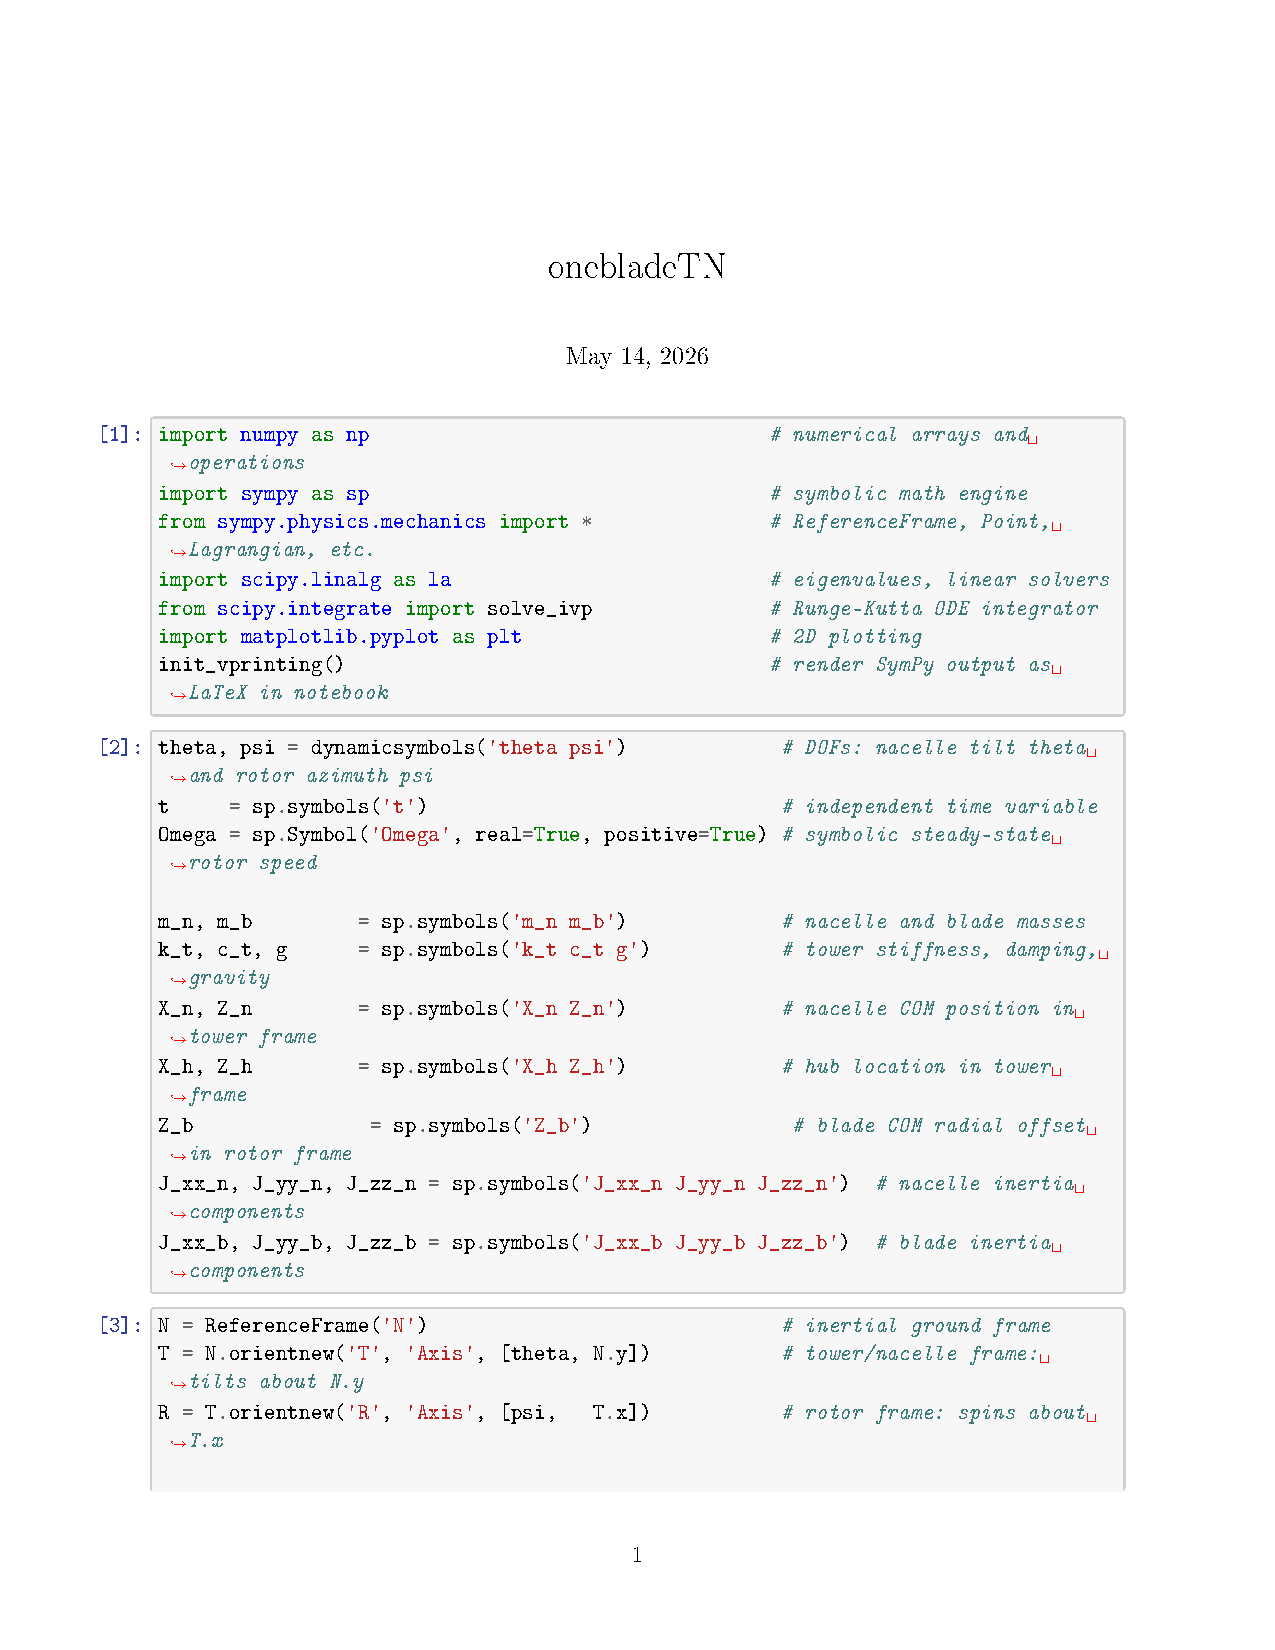
\includepdf[
    pages={1}, 
    scale=0.9, 
    pagecommand={%
        \thispagestyle{plain}%
        \subsection{Rigid Rotating Blade, Tilting Nacelle code}\label{app:RRBTNcode}%
    }
]{onebladeTN.pdf}

\includepdf[
    pages={2-}, 
    scale=0.9, 
    pagecommand={\thispagestyle{plain}}
]{onebladeTN.pdf}

\clearpage
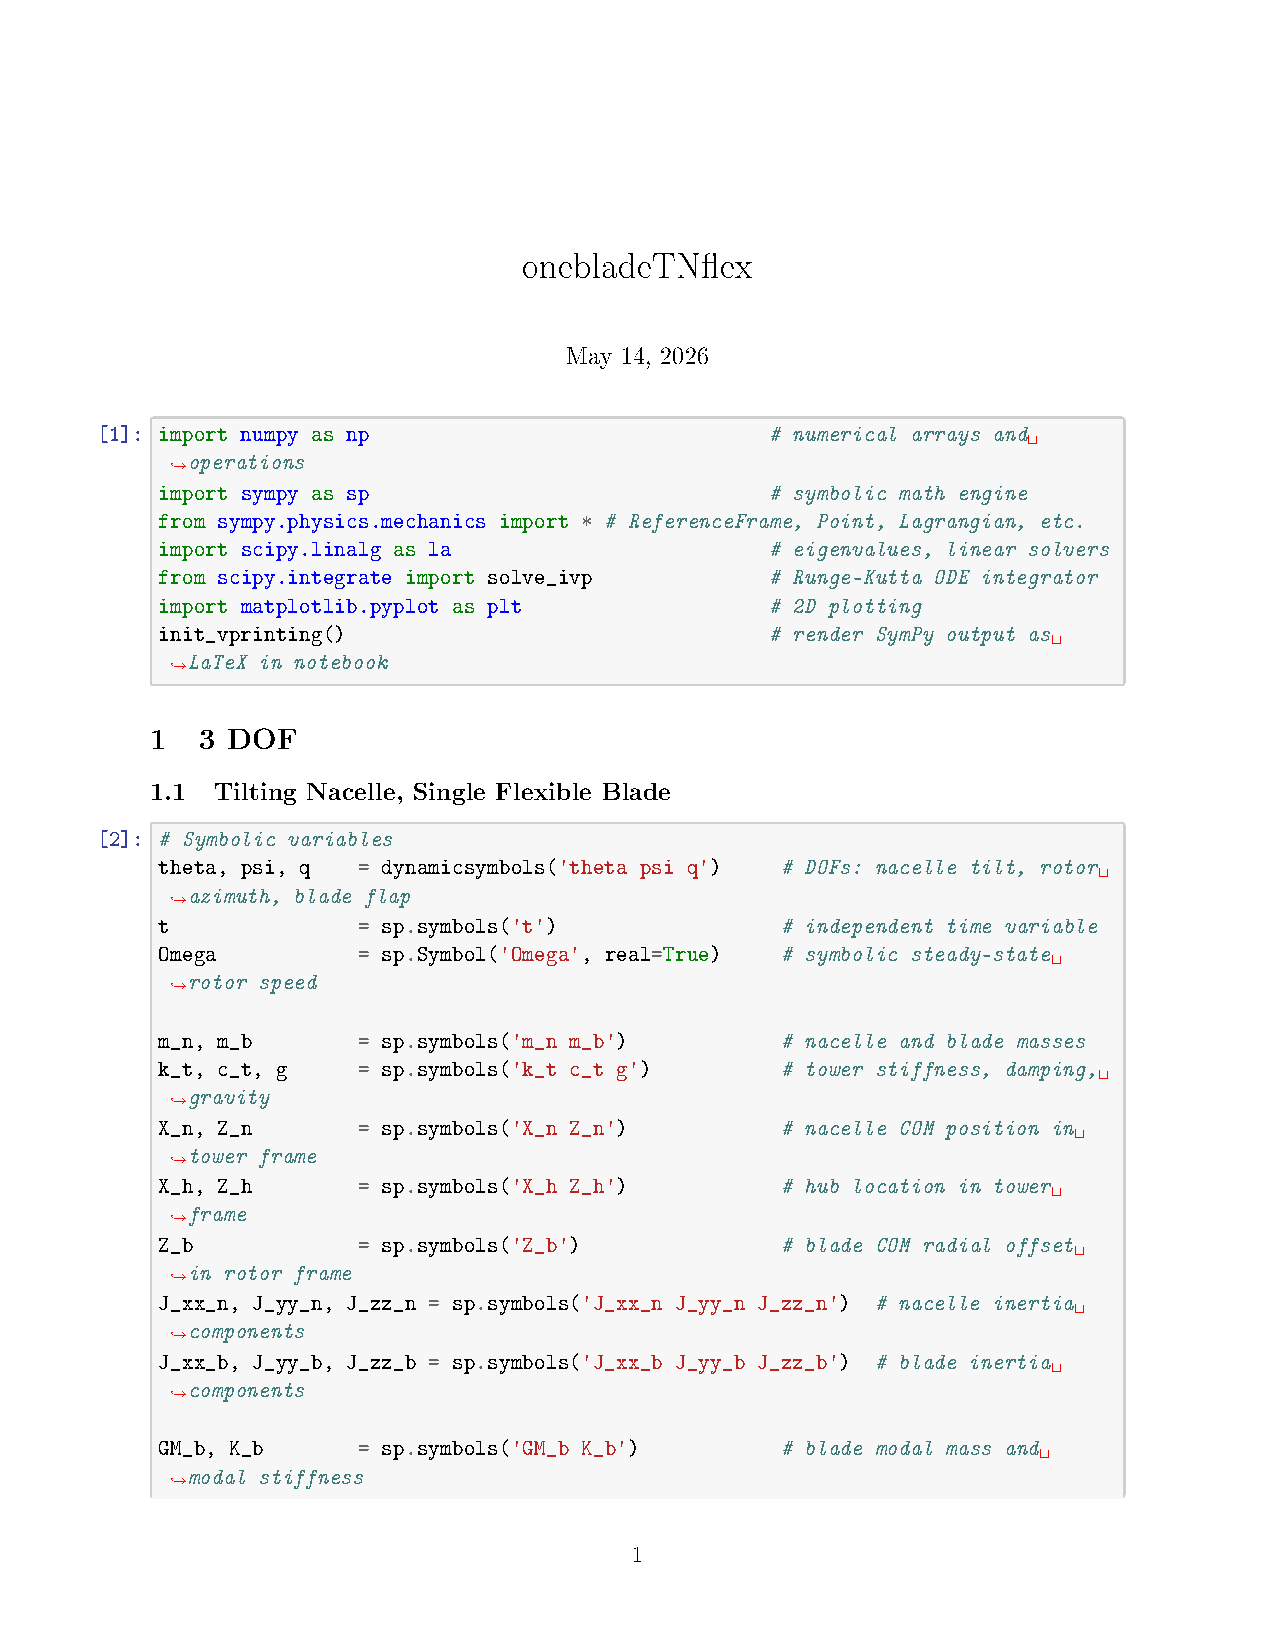
\includepdf[
    pages={1}, 
    scale=0.9, 
    pagecommand={%
        \thispagestyle{plain}%
        \subsection{Flexible Rotating Blade, Tilting Nacelle code}\label{app:FRBTNcode}%
    }
]{onebladeTNflex.pdf}

\includepdf[
    pages={2-}, 
    scale=0.9, 
    pagecommand={\thispagestyle{plain}}
]{onebladeTNflex.pdf}

% --- Bibliography Section ---
\newpage
\bibliography{references}
\end{document}